
%%%%%%%%%%%%%%%%%%%%%%%%%%%%%%%%%%%%%%%%%%%%%%%%%%%%%%%%%%%%%%%%%%%%%%%%%%%%%%%
% Author:  Pablo Alvarado
%
% Área Académica de Ingeniería en Computadores
% Instituto Tecnológico de Costa Rica
%
% Tesis de Licenciatura
% 
% Phone:   +506 2550 2495
% email:   palvarado@tec.ac.cr
%
%%%%%%%%%%%%%%%%%%%%%%%%%%%%%%%%%%%%%%%%%%%%%%%%%%%%%%%%%%%%%%%%%%%%%%%%%%%%%%%

% \documentclass is book

% If you want a printable two-side version of the thesis
%\documentclass[12pt,twoside,letterpaper]{book}

% If you want an electronic-only version of the thesis, do it one-sided
\documentclass[12pt,oneside,letterpaper]{book}

\usepackage[utf8]{inputenc}
\usepackage{ifthen}                     % provide if-then-else operators
\usepackage[backend=biber]{biblatex}
\usepackage{float}
\usepackage{listings}
\usepackage{pdfpages}
\usepackage{graphicx}

%Code listing style named "mystyle"
\lstdefinestyle{mystyle}{
  backgroundcolor=\color{white},   commentstyle=\color{codegreen},
  keywordstyle=\color{purple},
  numberstyle=\tiny\color{codegray},
  stringstyle=\color{codepurple},
  basicstyle=\ttfamily\footnotesize,
  breakatwhitespace=false,         
  breaklines=true,                 
  captionpos=b,                    
  keepspaces=true,                 
  numbers=left,                    
  numbersep=5pt,                  
  showspaces=false,                
  showstringspaces=false,
  showtabs=false,                  
  tabsize=1
}

%"mystyle" code listing set
\lstset{style=mystyle}
% \addbibresource{references.bib}

% --------------------------------------------------------------------------
% Global variables required in document formatting
% --------------------------------------------------------------------------
%
% BOOK MODE
%
\newboolean{bookmode}                  % boolean used to control book format
% Ensure that only one of the next two lines is active:
\setboolean{bookmode}{true}           % turn book mode on
%\setboolean{bookmode}{false}           % turn book mode off

%
% DRAFT MODE
%   The draft mode activates the TODO index and some "draft" markings all
%   around.  Ensure you set it to false for the final version!!
%
\newboolean{draftmode}                  % boolean used to control draft-mode
% Ensure that only one of the next two lines is active:
%\setboolean{draftmode}{true}            % turn draft mode on
\setboolean{draftmode}{false}           % turn draft mode off
% --------------------------------------------------------------------------
%
% GENERAL AUTHOR, TITLE AND KEYWORDS
%
% Nombre del Estudiante
\newcommand{\thesisAuthorAddress}{el señor} %% el señor / la señora / ...
\newcommand{\thesisAuthor}{Esteban Calvo Vargas} %% Nombre completo
\newcommand{\thesisAuthorShort}{E.~Calvo}  %% Nombre corto para pie de página
\newcommand{\thesisAuthorTECID}{201270170} %% Carné

% Título de la tesis
\newcommand{\thesisTitle}{Approximate kernel generation for convolutional neural networks using OpenCL}

% Keywords
\newcommand{\thesisKeywordsES}{computación aproximada, \textit{hardware} aproximado,
FPGA, aprendizaje profundo, OpenCL, \textit{High-level Synthesis}}

% Keywords
\newcommand{\thesisKeywordsEN}{approximate computing, approximate hardware,
FPGA, deep learning, OpenCL, High-level Synthesis}

% Descripción de la editorial
\newcommand{\boxeditorial}{%
}

% --------------------------------------------------------------------------

% include all packages and define all required general macros
%%%%%%%%%%%%%%%%%%%%%%%%%%%%%%%%%%%%%%%%%%%%%%%%%%%%%%%%%%%%%%%%%%%%%%%%%%%%%%%
% Author:  Pablo Alvarado
%
% Escuela de Electrónica
% Instituto Tecnológico de Costa Rica
%
% Phone:   +506 550 2106
% Fax:     +506 591 6629
% email:   palvarado@ietec.org
%
% $Id: macros.tex 1497 2010-08-09 17:04:26Z palvarado $
%
%%%%%%%%%%%%%%%%%%%%%%%%%%%%%%%%%%%%%%%%%%%%%%%%%%%%%%%%%%%%%%%%%%%%%%%%%%%%%%%

% Configuration of the exercises package, which is used to collect all
% problems and answers in the document.
\usepackage[exercisedelayed,answerdelayed,lastexercise]{exercise}
\renewcounter{Exercise}[chapter]
\renewcommand{\ExerciseName}{Problema}
\renewcommand{\theExercise}{\thechapter.\arabic{Exercise}}
\newcommand{\ExerciseLabel}{Exercise.\theExercise}
\renewcommand{\ExerciseHeader}%
{\textbf{\ExerciseName\ \theExercise.\ \ExerciseHeaderTitle\ }}
\renewcommand{\AnswerHeader}%
{\textbf{\ExerciseName\ \theExercise.\ }}


\usepackage{ifpdf}

% Command to change between draft or release mode:
\newcommand{\ifdraft}[2]{\ifthenelse{\boolean{draftmode}}{#1}{#2}}
% Command to change between draft or release mode:
\newcommand{\ifbook}[2]{\ifthenelse{\boolean{bookmode}}{#1}{#2}}

% include all required packages here
\usepackage{csquotes}                     % recommended for biblatex
\usepackage[english]{babel}               % supports english, but default is 
                                          % spanish...
% \newcommand*{\SelectSpanish}{%          % well, the last line indeed selects
%   \hyphenrules{spanish}%                % english over spanish, but with this
%   \languageshorthands{spanish}%         % command we turn it around.
%   \captionsspanish                      % The reason: hyperref has some
%   \datespanish                          % problems with the spanish babel,
% }                                       % so we use some trick here so that it
% \AtBeginDocument{\SelectSpanish}        % thinks it is english.

\usepackage{makeidx}                    % to create index file

\ifdraft{%
  %\usepackage[refpage]{nomencl}        % Use to easily administrate the list
 \usepackage{nomencl}                   % of symbols
}{%
 \usepackage{nomencl}
}
%\usepackage{times}                     % replace latex pk fonts with ps type I
                                        % don't forget to use dvips -D600 -Pcmz
                                        % to ensure Type I fonts!
\usepackage{amsmath}
\usepackage{amssymb,amstext}            % AMS-math and symbols package
\usepackage{mathrsfs}                   % Calygraphic fonts for transforms
\usepackage{array}                      % extensions to tabular environment
\usepackage{longtable}                  % supports extraordinary long tables
\usepackage{tabularx}                   % supports tables with fixed width
\usepackage{afterpage}                  % put something only after the page
\usepackage{multirow}                   % supports multiple row grouping in 
                                        % tables
\usepackage{multicol}                   % multiple columns environments
%\usepackage{paralist}                  % a few enumeration settings (old)
\usepackage{enumitem}                   % better enumeration with paralist 
                                        % equivalents as follows:

\newlist{compactitem}{itemize}{3}
\setlist[compactitem]{topsep=0pt,partopsep=0pt,itemsep=0pt,parsep=0pt}
\setlist[compactitem,1]{label=\textbullet}
\setlist[compactitem,2]{label=---}
\setlist[compactitem,3]{label=*}

\newlist{compactdesc}{description}{3}
\setlist[compactdesc]{topsep=0pt,partopsep=0pt,itemsep=0pt,parsep=0pt}

\newlist{compactenum}{enumerate}{3}
\setlist[compactenum]{topsep=0pt,partopsep=0pt,itemsep=0pt,parsep=0pt}

\usepackage{icomma}                     % decimal comma in math mode

\usepackage{bold-extra}

\usepackage[format=hang,%
            font=small,%
            labelfont=bf]{caption}      % nicer figure captions
%\usepackage{sty/ftcap}                 % switch \abovecaptionskip and
%                                       % \belowcaptionskip for tables, in 
%                                       % order to avoid the caption to be
%                                       % too near to the table itself
% locally added packages
\usepackage{float}                      % really place figures "here" (H)
\usepackage{booktabs}                   % book type tabulars

% the own style with options depending on the draft mode
\ifdraft{%
\usepackage[todo]{sty/tecStyle}         % some command definitions
                                        % options [todo] todo-index
}{%
\usepackage{sty/tecStyle}               % some command definitions
                                        % options [todo] todo-index
}


%% fix the title for examples
\renewcommand{\examplelistname}{Índice de ejemplos}
\renewcommand{\examplename}{Ejemplo}

%% define some command to cope with the tribunal names

%% Lector I

\newcommand{\nameLectorI}{$<$\emph{Use setLectorI in main.tex}$>$}
\newcommand{\genderLectorI}{$<$\emph{Use setLectorI in main.tex}$>$}

\newcommand{\setLectorI}[1][M]{%
  \ifthenelse{\equal{#1}{F}}{%
    \renewcommand{\genderLectorI}{Profesora Lectora}%
  }{%
    \renewcommand{\genderLectorI}{Profesor Lector}
  }
  \lectorIRelay
}

\newcommand{\lectorIRelay}[1]{%
  \renewcommand{\nameLectorI}{#1}
}

%% Lector II

\newcommand{\nameLectorII}{$<$\emph{Use setLectorII in main.tex}$>$}
\newcommand{\genderLectorII}{$<$\emph{Use setLectorII in main.tex}$>$}

\newcommand{\setLectorII}[1][M]{%
  \ifthenelse{\equal{#1}{F}}{%
    \renewcommand{\genderLectorII}{Profesora Lectora}%
  }{%
    \renewcommand{\genderLectorII}{Profesor Lector}
  }
  \lectorIIRelay
}

\newcommand{\lectorIIRelay}[1]{%
  \renewcommand{\nameLectorII}{#1}
}

%% Asesor

\newcommand{\nameAsesor}{$<$\emph{Use setAsesor in main.tex}$>$}
\newcommand{\genderAsesor}{$<$\emph{Use setAsesor in main.tex}$>$}

\newcommand{\setAsesor}[1][M]{%
  \ifthenelse{\equal{#1}{F}}{%
    \renewcommand{\genderAsesor}{Profesora Asesora}%
  }{%
    \renewcommand{\genderAsesor}{Profesor Asesor}
  }
  \asesorRelay
}

\newcommand{\asesorRelay}[1]{%
  \renewcommand{\nameAsesor}{#1}
}





\usepackage{url}                        % allows linebreaks at certain
                                        % characters or combinations of 
                                        % characters for URLs

\usepackage[nottoc]{tocbibind}          % Fix the hyperrefs to TOC,TOF, etc.
                                        % and ensure that they appear all in 
                                        % the Table of Contents

% For pdflatex
% - The hyperref package should always be loaded last, since it has to
%   overwrite some of the commands.
% - The package subfigure caused that the pagebackrefs and index refs were set
%   incorrectly.

\ifpdf
%
% final / draft document options
\usepackage{graphicx}                   % for inserting pdf-graphics.
                                        % options final / draft
\ifdraft{%
% Use biber/biblatex
\usepackage[backend=biber,
            style=ieee,
            sorting=nyt,
            backref=true,
           ]{biblatex}

\usepackage[%pdftex,%
            naturalnames=true,
            linktocpage,
            hyperindex,
            colorlinks,
            urlcolor=dkred,          %\href to external url
            filecolor=dkmagenta,     %\href to local file
            linkcolor=dkred,         %\ref and \pageref
            citecolor=dkgreen,       %\cite
            plainpages=false,
            pdfpagelabels,
            pdfpagemode=UseOutlines, % means use bookmarks (None,UseOutlines)
            % bookmarksopen=false,   % would show the whole hierarchy if true
            bookmarksnumbered=true,
            pdfpagelayout=OneColumn, % SinglePage,OneColumn,TwoColumnLeft,...
            pdfview=FitH, % FitB,FitBH,FitBV,Fit,FitH,FitV
            pdfstartview=FitH, % FitB,FitBH,FitBV,Fit,FitH,FitV
            ]{hyperref}
}{%
% Use biber/biblatex
\usepackage[backend=biber,
            style=ieee,
            sorting=nyt
           ]{biblatex}

\usepackage[%pdftex,%
            naturalnames=true,
            linktocpage,hyperindex,
            colorlinks,
            urlcolor=dkred,          %\href to external url
            filecolor=dkmagenta,     %\href to local file
            linkcolor=dkred,         %\ref and \pageref
            citecolor=dkgreen,       %\cite
            plainpages=false,
            pdfpagelabels,
            pdfpagemode=UseOutlines, % means use bookmarks (None,UseOutlines)
            % bookmarksopen=false,   % open the whole hierarchy if true!
            bookmarksnumbered=true,
            pdfpagelayout=OneColumn, % SinglePage,OneColumn,TwoColumnLeft,...
            pdfview=FitH, % FitB,FitBH,FitBV,Fit,FitH,FitV
            pdfstartview=FitH, % FitB,FitBH,FitBV,Fit,FitH,FitV
            ]{hyperref}
}


%
% Ensure that the links of the images point to the top of the images and not
% to the caption
%
\usepackage[figure]{hypcap}

% %
% % Ensure that pdfLaTeX do the same spacing as LaTeX
% %
\pdfadjustspacing=1 
% %
\else   % i.e. if not pdf

\usepackage[active]{srcltx}             % insert links into the dvi to jump
\usepackage{graphicx}                   % for inserting eps-graphics.
                                        % options final / draft
                                        % into the sources directly.
\ifdraft{%
% Use biber/biblatex
\usepackage[backend=biber,
            style=ieee,
            sorting=nyt,
            backref=true,
           ]{biblatex}

\usepackage[ps2pdf,%
            % plainpages=false,
            linktocpage,
            hyperindex,
            % pdfpagelabels,
            pdfpagemode=UseOutlines,
            pdfstartview=FitH]{hyperref}
}{%
% Use biber/biblatex
\usepackage[backend=biber,
            style=ieee,
            sorting=nyt
           ]{biblatex}
\usepackage[ps2pdf,%
            % plainpages=false,
            linktocpage,
            hyperindex,
            % pdfpagelabels,
            pdfpagemode=UseOutlines,
            pdfstartview=FitH]{hyperref}
}

%\usepackage[ps2pdf]{hyperref}

\fi  % end of if pdf or not

% --------------------------------------------------------------------------

% Allow the use of international characters
\AtBeginDocument{%
  \hypersetup{%
             pdftitle={\thesisTitle},%
             pdfsubject={Tesis de Licenciatura},%
             pdfauthor={\thesisAuthor},%
             pdfkeywords={\thesisKeywords}
            }%
}


%\usepackage{sty/algorithmic}            % algorithmic environment


\usepackage{rotating}                   % allow block rotation


%%%%%%%%%%%%%%%%%%%%%%%%%%%%%%%%%%%%%%%%%%%%%%%%%%%%%%%%%%%%%%%%%%%%%%%%%%%%%%%

%\sloppy

%
% Some own font definitions
%
\DeclareMathAlphabet{\mathpzc}{OT1}{pzc}{m}{it}
\DeclareMathAlphabet{\mathpss}{OT1}{cmss}{m}{sl}

%
% page layout
%

\usepackage{vmargin}
\setpapersize{USletter}

% For letter-paper printing
\setmarginsrb{33mm}{8mm}{23mm}{7mm}{15pt}{15pt}{7mm}{12mm}
%\setlength{\headheight}{15pt}         % fancy headers wanted this

%
% Fraction of Float Object / Text
%

\renewcommand{\topfraction}{0.95}       % how much of top of page should be 
                                        % allowed to be float object?
\renewcommand{\bottomfraction}{0.95}    % how much of bottom of page should be
                                        % allowed to be float object?
\renewcommand{\textfraction}{0.05}      % how much of page must be text?

\usepackage{fancyhdr}                   % fancy page headers

\usepackage{lastpage}

%
% header and footer layout (needs package fancyhdr)
%
\newcommand{\copyrightfooter}{\tiny{\copyright \the\year ---
    \thesisAuthorShort \qquad Uso exclusivo ITCR}}
%
\newcommand{\draftfoot}%
  {\ifdraft{\textcolor{dkblue}{\tiny\textsl{Borrador: \today}}{}}
           {}
}

\pagestyle{fancy}
\renewcommand{\chaptermark}[1]{\markboth{{\small
    \thechapter\hspace*{1mm}#1}}{}}
\renewcommand{\sectionmark}[1]{\markright{{\small
    \thesection\hspace*{1mm}#1}}{}}
%\lhead[{\small\textsc\Roman{\thepage}}]{\fancyplain{}%
\lhead[{\small\thepage}]{\fancyplain{}%
        {{\slshape \small\nouppercase{\leftmark}}}}
\chead[]{}
\rhead[\fancyplain{}%
%        {{\slshape \small\nouppercase{\rightmark}}}]{{\small\textsc\Roman{\thepage}}}
        {{\slshape \small\nouppercase{\rightmark}}}]{{\small\thepage}}
\lfoot[]{\draftfoot}
\ifbook{%
  \cfoot[]{}
}{
  \cfoot[\copyrightfooter]{\copyrightfooter}
}
\rfoot[\draftfoot]{}
\renewcommand{\headrulewidth}{0.5pt}
\renewcommand{\footrulewidth}{0pt}

%
% Caption style for tables
% Requires the packages caption2 and ftcap
% (caption2 required this, but is obsolete now:)
%
%\newcaptionstyle{tablecaptionstyle}{%
%  \renewcommand\captionlabelfont{\normalsize\bf}
%  \renewcommand\captionfont{\normalsize}
%  \usecaptionstyle{hang}%
%}

% For caption v3:
\captionsetup[table]{position=top,format=hang,textfont={normalsize},labelfont={normalsize,bf}}

\newcommand{\tablecaption}[2][foo]{%
  \ifthenelse{\equal{#1}{foo}}{%
    %\captionstyle{tablecaptionstyle}%
    \caption{#2}%
  }
  {%
    %\captionstyle{tablecaptionstyle}%
    \caption[#1]{#2}%
  }
}
% \addto\extrasspanish{\renewcommand{\tablename}{Tabla}}
% \addto\extrasspanish{\renewcommand{\listtablename}{\'Indice de tablas}}

%
% paragraph layout
%
\renewcommand{\baselinestretch}{1.1}    % line spacing
\parindent0em                           % indentation width of first line
\parskip1.3ex                           % space between paragraphs

%
% document consists of
% chapter - section - subsection - subsubsection - paragraph - subparagraph
%
\setcounter{secnumdepth}{2}             % depth of section numbering
\setcounter{tocdepth}{2}                % depth of table of contents

% For biblatex
\addbibresource{literatura.bib}

%
% prepares index from entries like \index{word} or \index{group!word}.
% don't forget to call "makeindex filename" for final index generation.
%
\makeindex                            %% for package makeidx.sty
%\newindex{default}{idx}{ind}{Index}  %% for package index.sty

\newcommand{\octave}{GNU/Octave}


%
% prepares notation or nomenclature 
%
%\makeglossary
\makenomenclature

%%% Local Variables: 
%%% mode: latex
%%% TeX-master: "main"
%%% End: 


% Tribunal Evaluador
%
% Indique los nombres de los lectores y asesor
% El parámetro opcional es [M]asculino o [F]emenino
\setLectorI[F]{Dra.\, María del Pilar Pérez Fernández}
\setLectorII{M.\,Sc.\,Juan Pérez Hernández}
\setAsesor{Ing.\,Albert Einstein Sánchez}

% allow equations to be splitted (breaked) into several pages
\allowdisplaybreaks[3]

% --------------------------------------------------------------------------
\begin{document}
  % where to look for graphics
  \graphicspath{{./}{./fig/}}

  \pagenumbering{alph}
  % fix some terms not activated due to the bug of hyperref with spanish.
  \renewcommand{\tablename}{Table}
  % \renewcommand{\listtablename}{Table index}
  \renewcommand{\listtablename}{List of Tables}
  \renewcommand{\examplesolution}{Solution}
  \pagestyle{empty}

  % select one of the following titlepages
  %%% ---------------------------------------------------------------------------
%% titlepage_licce_es.tex
%%
%% Title page
%%
%% $Id: titlepage.tex 1452 2010-07-07 00:55:16Z palvarado $
%% ---------------------------------------------------------------------------

\thispagestyle{empty} 

\begin{center}

Tecnológico de Costa Rica

\par\vspace{1ex}

Computer Engineering Academic Area

\par\vspace{1ex}

Licentiate Degree Program in Computer Engineering

\par\vspace{20mm}


\includegraphics[width=60mm]{Firma_TEC-4}

\par\vspace*{\fill}

{\large\bf{\thesisTitle}}

\par\vspace*{\fill}

Report of Graduation Work in fulfillment of the requirements for the degree

of Licentiate in Computer Engineering

\par\vspace{20mm}

\thesisAuthor

\vspace*{\fill}

\ifdraft{%
{Borrador de \today}
}{
Cartago, November, 2019
}
\end{center}
\newpage 
\cleardoublepage 


%%% Local Variables: 
%%% mode: latex
%%% TeX-master: "main"
%%% End: 
 % Titlepage in Spanish

  %%% ---------------------------------------------------------------------------
%% titlepage_licce_es.tex
%%
%% Title page
%%
%% $Id: titlepage.tex 1452 2010-07-07 00:55:16Z palvarado $
%% ---------------------------------------------------------------------------

\thispagestyle{empty} 

\begin{center}

Tecnológico de Costa Rica

\par\vspace{1ex}

Área Académica de Ingeniería en Computadores

\par\vspace{1ex}

Programa de Licenciatura de Ingeniería en Computadores

\par\vspace{20mm}


\includegraphics[width=60mm]{Firma_TEC-4}

\par\vspace*{\fill}

{\large\bf{\thesisTitle}}

\par\vspace*{\fill}

Informe de Trabajo Final de Graduación para optar por el título de

Ingeniero en Computadores con el grado académico de Licenciatura

\par\vspace{20mm}

\thesisAuthor

\vspace*{\fill}

\ifdraft{%
{Borrador de \today}
}{
Cartago, 7 de marzo, 2018
}
\end{center}
\newpage 
\cleardoublepage 


%%% Local Variables: 
%%% mode: latex
%%% TeX-master: "main"
%%% End: 
  % Titlepage in Spanish
  %% ---------------------------------------------------------------------------
%% titlepage_licce_es.tex
%%
%% Title page
%%
%% $Id: titlepage.tex 1452 2010-07-07 00:55:16Z palvarado $
%% ---------------------------------------------------------------------------

\thispagestyle{empty} 

\begin{center}

Tecnológico de Costa Rica

\par\vspace{1ex}

Computer Engineering Department

\par\vspace{1ex}

Licentiate Degree Program in Computer Engineering

\par\vspace{20mm}


\includegraphics[width=60mm]{Firma_TEC-4}

\par\vspace*{\fill}

{\large\bf{\thesisTitle}}

\par\vspace*{\fill}

Final report submitted in partial fulfillment of the requirements
for the degree of Licentiate in Computer Engineering

\par\vspace{20mm}

\thesisAuthor

\vspace*{\fill}

\ifdraft{%
{Draft \today}
}{
% Cartago, March 7th, 2018
Cartago, \today
}
\end{center}
\newpage 
\cleardoublepage 


%%% Local Variables: 
%%% mode: latex
%%% TeX-master: "main"
%%% End: 
 % Titlepage in English (only if thesis is in En)
  
  %%% ---------------------------------------------------------------------------
%% titlepage_msc_es.tex
%%
%% Title page
%%
%% $Id: titlepage.tex 1452 2010-07-07 00:55:16Z palvarado $
%% ---------------------------------------------------------------------------

\thispagestyle{empty} 

\begin{center}

Tecnológico de Costa Rica

\par\vspace{1ex}

Escuela de Ingeniería Electrónica

\par\vspace{20mm}


\includegraphics[height=60mm]{Firma_TEC-4}

\par\vspace*{\fill}

{\large\bf{\thesisTitle}}

\par\vspace*{\fill}

Documento de tesis sometido a consideración para optar por el grado
académico de Maestría en Electrónica con Énfasis en
%
%Sistemas Embebidos
Procesamiento Digital de Señales
%Microelectrónica
%Sistemas Microelectromecánicos

\par\vspace{20mm}

\thesisAuthor

\vspace*{\fill}

\ifdraft{%
{Borrador de \today}
}{
Cartago, 19 de noviembre, 2013
}
\end{center}
\newpage 
\cleardoublepage 


%%% Local Variables: 
%%% mode: latex
%%% TeX-master: "main"
%%% End: 
   % Titlepage in Spanish
  %%% ---------------------------------------------------------------------------
%% titlepage.tex
%%
%% Title page
%%
%% $Id: titlepage.tex 1452 2010-07-07 00:55:16Z palvarado $
%% ---------------------------------------------------------------------------

\thispagestyle{empty} 

\begin{center}

Tecnológico de Costa Rica

\par\vspace{1ex}

Escuela de Ingeniería Electrónica

\par\vspace{20mm}


\includegraphics[height=60mm]{Firma_TEC-4}

\par\vspace*{\fill}

{\large\bf{\thesisTitle}}

\par\vspace*{\fill}

A thesis submitted in partial fulfillment of the requirements for the
degree of
%
Master of Science in Electronics, Major in 
%
%Embedded Systems
Digital Signal Processing
%Microelectronics
%Microelectromechanical systems

\par\vspace{20mm}

\thesisAuthor

\vspace*{\fill}

\ifdraft{%
{Draft \today}
}{
Cartago, November 19th, 2017
}
\end{center}
\newpage 
\cleardoublepage 


%%% Local Variables: 
%%% mode: latex
%%% TeX-master: "main"
%%% End: 
   % Titlepage in English (only if thesis is in En)

  % \thispagestyle{empty}

\rule{10mm}{0pt}

\vfill

Declaro que el presente documento de tesis ha sido realizado enteramente
por mi persona, utilizando y aplicando literatura referente al tema e
introduciendo conocimientos y resultados experimentales propios.

En los casos en que he utilizado bibliografía he procedido a indicar las
fuentes mediante las respectivas citas bibliográficas.  En consecuencia,
asumo la responsabilidad total por el trabajo de tesis realizado y por
el contenido del presente documento.



\vspace*{8mm}

\begin{flushright}
  \thesisAuthor\par
  Cartago, \today\par
  Céd: 1-0123-0456
\end{flushright}

\cleardoublepage

%%% Local Variables: 
%%% mode: latex
%%% TeX-master: "main"
%%% End: 


  % 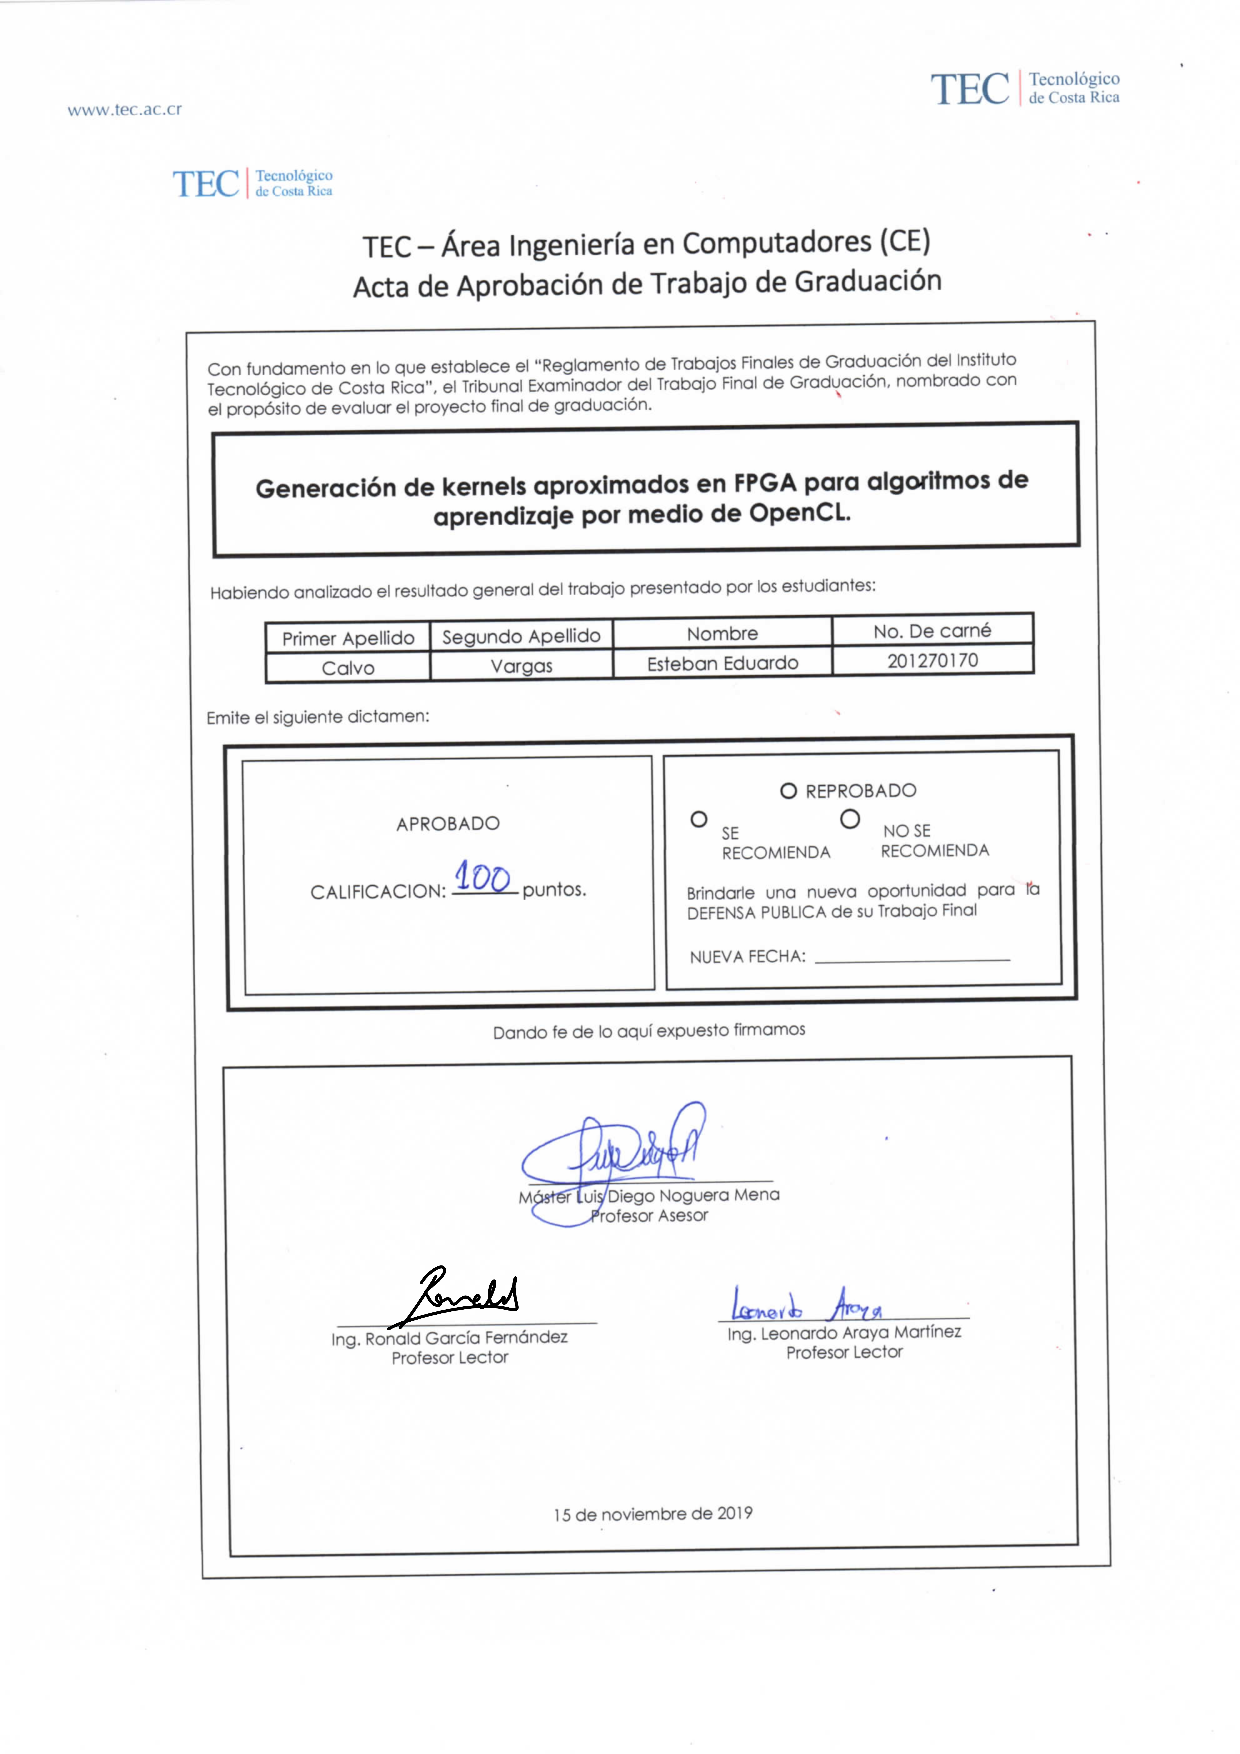
\includepdf[page={1}]{acta}
  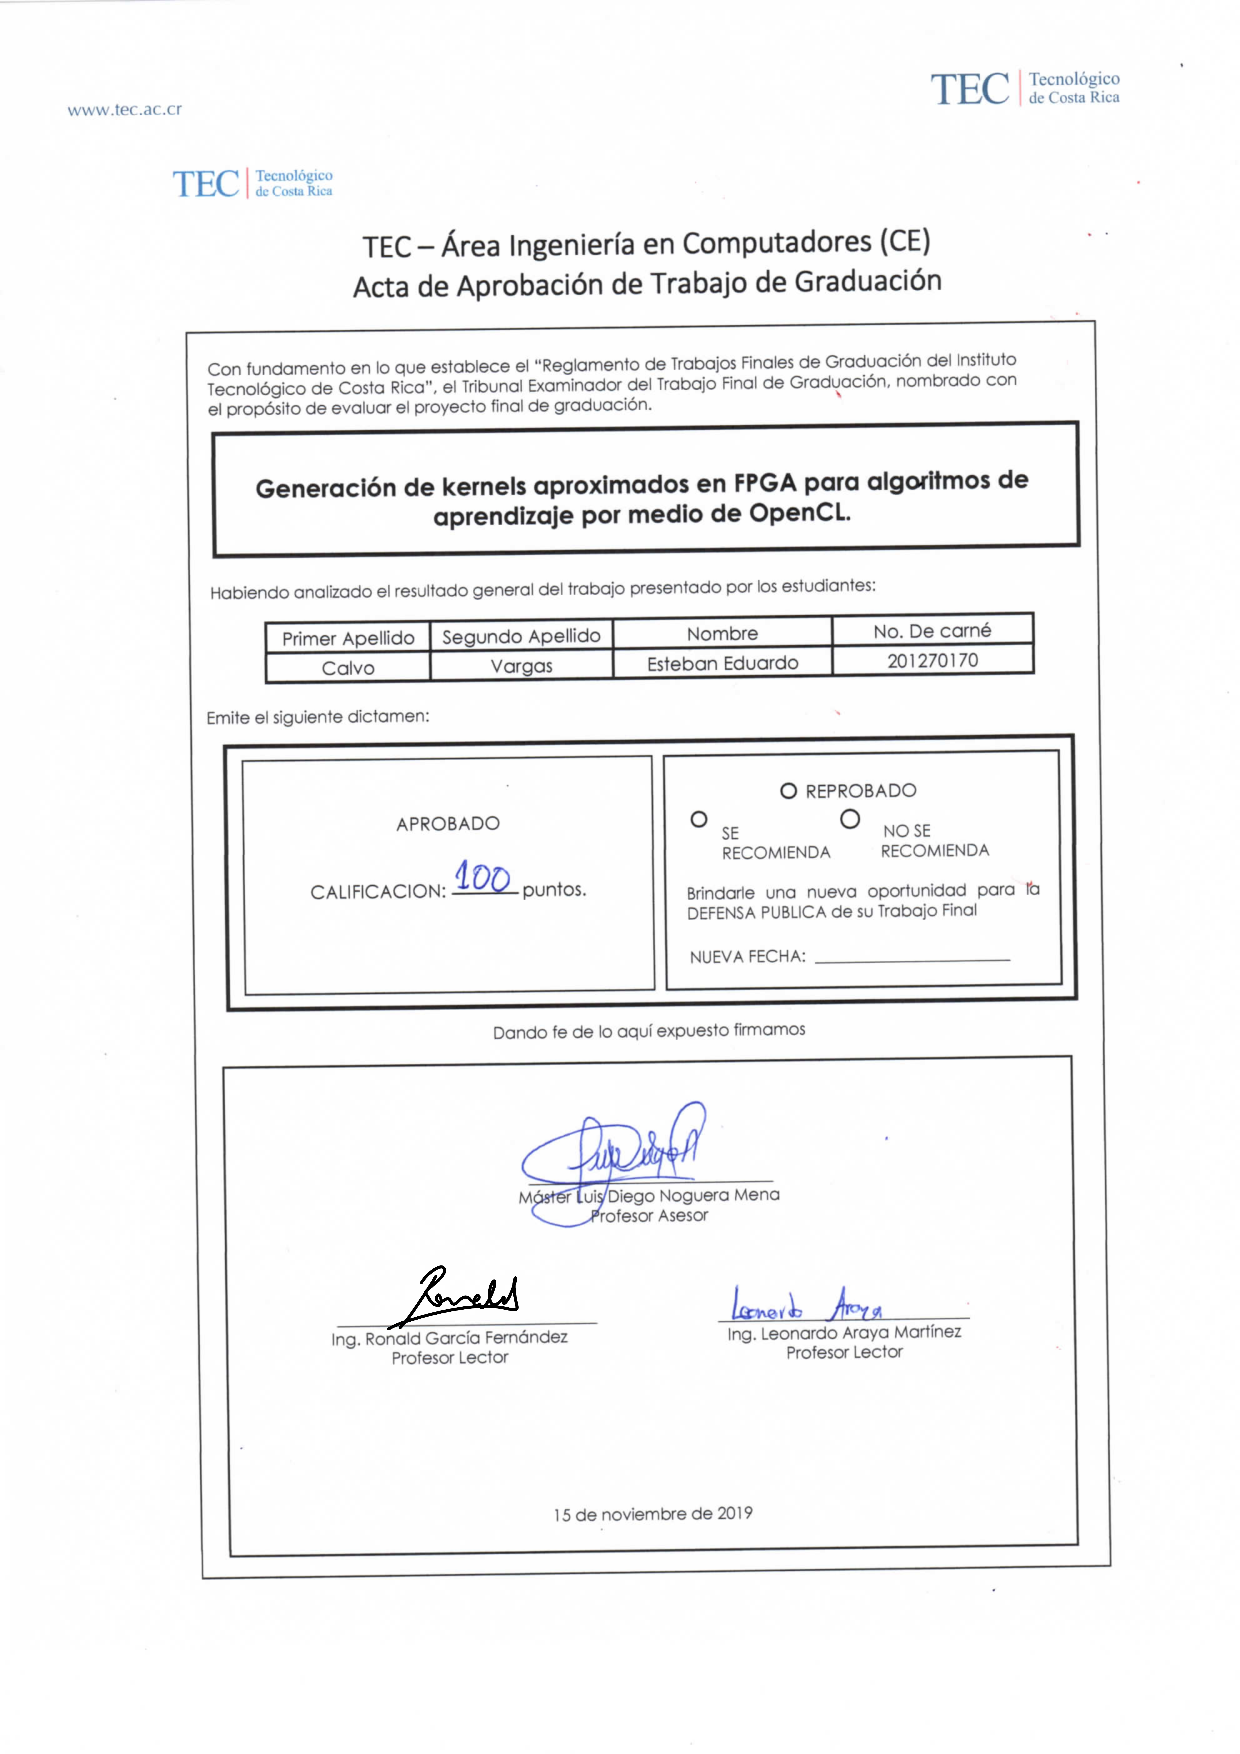
\includegraphics[width=\linewidth,page=1]{acta}

  \vspace*{0.4\textheight}
{\hfill{\Large{\emph{a mis queridos padres}}}}

  \chapter*{Agradecimientos}
\thispagestyle{empty}

Gratitude pending

\vspace*{1cm}

\thesisAuthor

San Jose, \today

\cleardoublepage

%%% Local Variables: 
%%% mode: latex
%%% TeX-master: "paMain"
%%% End: 

  \chapter*{Resumen}
\thispagestyle{empty}

El uso de FPGAs para la aceleraci\'on de aplicaciones
de aprendizaje de m\'aquina es un área en desarollo
debido al alto nivel de especialización de este tipo de
plataformas. Otra técnica de aceleración de aplicaciones
es la computación aproximada. El presente trabajo muestra
técnicas de computación aproximada siendo utilizadas para
dirigir el diseño de una implementación en FPGA de redes
neuronales convolucionales por medio de OpenCL, una
herramienta para la definición de procesos en plataformas
heterogéneas. Se demuestra cómo la combinación
de ambas técnicas puede llevar a ganancias significativas
en tiempo de ejecución y uso de recursos de la plataforma
con pequeñas pérdidas en exactitud.

\bigskip

\textbf{Palabras clave:} \thesisKeywordsES

\clearpage
\chapter*{Abstract}
\thispagestyle{empty}

The use of FPGAs for accelerating machine learning applications
is a research area due to the high specialization level of
this type of platforms. Another technique for application
acceleration is approximate computing. The current work shows
approximate computing techniques being used to guide the
design of an approximate CNN implementation on an FPGA
through the use of OpenCL, a framework for process definition
on heterogenous platforms. It is shown how the combination
of both techniques can lead to significant gains on execution
time and resource usage with little losses on accuracy.

\bigskip

\textbf{Keywords:} \thesisKeywordsEN

\cleardoublepage

%%% Local Variables: 
%%% mode: latex
%%% TeX-master: "main"
%%% End: 

  
  %% -------------------------------------------------
  %% Acta y hoja del tribunal
  
  %% Para la licenciatura en electrónica:
  % %% ESTE ARCHIVO DEBE ELIMINARSE DE LA VERSIÓN FINAL

\thispagestyle{empty}

\begin{center}
  \begin{tabular}{c}
    Instituto Tecnológico de Costa Rica \\
    Escuela de Ingeniería Electrónica \\
    Proyecto de Graduación \\
    Acta de Aprobación
  \end{tabular}
\end{center}

\vfill

\begin{center}
  \begin{tabular}{c}
    Defensa de Proyecto de Graduación \\
    Requisito para optar por el título de Ingeniero en Electrónica \\
    Grado Académico de Licenciatura
  \end{tabular}
\end{center}

\vfill

%% \thesisAuthorAddress, \thesisAuthor y \thesisTitle están en main.tex
El Tribunal Evaluador aprueba la defensa del proyecto de graduación
denominado \textsl{\thesisTitle}, realizado por
%
\thesisAuthorAddress\ \thesisAuthor\ %
%
y, hace constar que cumple con las normas
establecidas por la Escuela de Ingeniería Electrónica del Instituto
Tecnológico de Costa Rica.

\vfill

\begin{center}
 Miembros del Tribunal Evaluador
\end{center}

\vfill

\begin{center}
  \begin{tabularx}{\textwidth}{cXc}
    \rule{0.45\textwidth}{0.5pt} && \rule{0.45\textwidth}{0.5pt} \\
    \nameLectorI                 && \nameLectorII \\
    \genderLectorI               && \genderLectorII
  \end{tabularx}
  
  \vspace{10mm}

  \begin{tabular}{c}
    \rule{0.45\textwidth}{0.5pt} \\
    \nameAsesor \\
    \genderAsesor
  \end{tabular}
\end{center}

\vfill

\begin{center}
  Cartago, \today\par
\end{center}

\cleardoublepage

%%% Local Variables: 
%%% mode: latex
%%% TeX-master: "main"
%%% End: 
  % Remover en versión final
  % %% ESTE ARCHIVO DEBE ELIMINARSE DE LA VERSIÓN FINAL


\thispagestyle{empty}

\begin{center}
  \begin{tabular}{c}
    Instituto Tecnológico de Costa Rica \\
    Escuela de Ingeniería Electrónica \\
    Proyecto de Graduación \\
    Tribunal Evaluador \\
    Acta de Evaluación
  \end{tabular}
\end{center}

\vfill

\begin{center}
  \begin{tabular}{c}
    Defensa de Proyecto de Graduación \\
    Requisito para optar por el título de Ingeniero en Electrónica \\
    Grado Académico de Licenciatura
  \end{tabular}
\end{center}

\vfill

%% \thesisAuthorAddress, \thesisAuthor y \thesisTitle están en main.tex
\begin{center}

  Estudiante:%
  \qquad \textbf{\thesisAuthor}%
  \qquad Carné: \thesisAuthorTECID

  \vspace*{2ex}

  \setlength\tabcolsep{0pt}
  \begin{tabular}{p{.25\textwidth}p{.73\textwidth}}
    Nombre del proyecto: & \textsl{\thesisTitle}
  \end{tabular}
\end{center}
\vspace{5mm}

\vfill

Los miembros de este Tribunal hacen constar que este proyecto de
graduación ha sido aprobado y cumple con las normas establecidas por
la Escuela de Ingeniería Electrónica del Instituto Tecnológico de
Costa Rica y es merecedor de la siguiente calificación:

\vfill

\begin{center}
  Nota de Proyecto de Graduación: \rule{25mm}{0.5pt}
\end{center}

\vfill

\begin{center}
 Miembros del Tribunal Evaluador
\end{center}

\vfill

% Defina con \setLector* en main.tex los lectores y asesor
\begin{center}
  \begin{tabularx}{\textwidth}{cXc}
    \rule{0.45\textwidth}{0.5pt} && \rule{0.45\textwidth}{0.5pt} \\
    \nameLectorI                 && \nameLectorII \\
    \genderLectorI               && \genderLectorII
  \end{tabularx}
  
  \vspace{10mm}

  \begin{tabular}{c}
    \rule{0.45\textwidth}{0.5pt} \\
    \nameAsesor \\
    \genderAsesor
  \end{tabular}
\end{center}

\vfill

\begin{center}
  Cartago, \today\par
\end{center}

\cleardoublepage

%%% Local Variables: 
%%% mode: latex
%%% TeX-master: "main"
%%% End: 
      % Remover en versión final
  
  %% Para la maestría en electrónica:
  %%% ESTE ARCHIVO DEBE ELIMINARSE DE LA VERSIÓN FINAL

\thispagestyle{empty}

\begin{center}
  \begin{tabular}{c}
    Instituto Tecnológico de Costa Rica \\
    Escuela de Ingeniería Electrónica \\
    Proyecto de Graduación \\
    Tesis de Maestría \\
    Tribunal Evaluador
  \end{tabular}
\end{center}

\vfill

Tesis de maestría defendida ante el presente Tribunal Evaluador como
requisito para optar por el grado académico de maestría, del Instituto
Tecnológico de Costa Rica.

\vfill

\vspace*{20mm}
\begin{center}
 Miembros del Tribunal
\end{center}
\vspace*{8mm}

\vfill

\begin{center}
  \begin{tabularx}{\textwidth}{cXc}
    \rule{0.45\textwidth}{0.5pt} && \rule{0.45\textwidth}{0.5pt} \\
    \nameLectorI                 && \nameLectorII \\
    \genderLectorI               && \genderLectorII
  \end{tabularx}
  
  \vspace{10mm}

  \begin{tabular}{c}
    \rule{0.45\textwidth}{0.5pt} \\
    \nameAsesor \\
    \genderAsesor
  \end{tabular}
\end{center}

\vfill


Los miembros de este Tribunal dan fe de que la presente tesis de maestría 
ha sido aprobada y cumple con las normas establecidas por la Escuela de
Ingeniería Electrónica.

\vfill

\begin{center}
  Cartago, \today\par
\end{center}

\cleardoublepage

%%% Local Variables: 
%%% mode: latex
%%% TeX-master: "main"
%%% End: 
  % Remover en versión final
  %%% ESTE ARCHIVO DEBE ELIMINARSE DE LA VERSIÓN FINAL


\thispagestyle{empty}

\begin{center}
  \begin{tabular}{c}
    Instituto Tecnológico de Costa Rica \\
    Escuela de Ingeniería Electrónica \\
    Tesis de Maestría \\
    Acta de Evaluación
  \end{tabular}
\end{center}

\vfill

Tesis de maestría defendida ante el presente Tribunal Evaluador como
requisito para optar por el grado académico de maestría, del Instituto
Tecnológico de Costa Rica.

\vspace*{15mm}

%% Definir \thesisAuthor, \thesisTitle, etc. en archivo main.tex
\begin{center}
  Estudiante: \thesisAuthor
\end{center}

\vfill

\begin{center}
  Nombre del Proyecto: \thesisTitle}
\end{center}

\vspace*{20mm}
\begin{center}
 Miembros del Tribunal Evaluador
\end{center}
\vspace*{8mm}

\vfill

% Los nombres de lectores y asesor se definen en el archivo main.tex
\begin{center}
  \begin{tabularx}{\textwidth}{cXc}
    \rule{0.45\textwidth}{0.5pt} && \rule{0.45\textwidth}{0.5pt} \\
    \nameLectorI                 && \nameLectorII \\
    \genderLectorI               && \genderLectorII
  \end{tabularx}
  
  \vspace{10mm}

  \begin{tabular}{c}
    \rule{0.45\textwidth}{0.5pt} \\
    \nameAsesor \\
    \genderAsesor
  \end{tabular}
\end{center}

\vfill

Los miembros de este Tribunal dan fe de que la presente tesis de
maestría ha sido aprobada y cumple con las normas establecidas por la
Escuela de Ingeniería Electrónica.

\vfill

\begin{center}
  Nota final de la Tesis de Maestría: \rule{3cm}{0.5pt}
\end{center}
\vfill

\begin{center}
  Cartago, \today\par
\end{center}

\cleardoublepage

%%% Local Variables: 
%%% mode: latex
%%% TeX-master: "main"
%%% End: 
      % Remover en versión final
  %% -------------------------------------------------
  

  %----------------------------------------------------------------------------
  \frontmatter
  %----------------------------------------------------------------------------
  \pagestyle{fancy}
  \pagenumbering{roman}

  \pdfbookmark[1]{Indice General}{Indice General}

  \parskip0ex                           % space between paragraphs

  \tableofcontents                      % Table of contents
  \listoffigures                        % List of figures
  \listoftables                         % List of tables

\ifdraft{%
  % todo's                              % TODOs
  \listoftodo
}{%
}

  %% ---------------------------------------------------------------------------
%% paNotation.tex
%%
%% Notation
%%
%% $Id: notation.tex 1467 2010-07-24 16:47:17Z palvarado $
%% ---------------------------------------------------------------------------

\newcommand{\nms}{\negmedspace}

%%
% Commands required for the nomenclature groups
%
% There are following prefix forms:
%  a   abbreviation    \syma[key]{symbol}{description}
%  g   general         \symg[key]{symbol}{description}
%%

\newcommand{\nmstyle}[1]{\large\item[\textbf{#1}]\normalsize}

\renewcommand{\nomgroup}[1]{%
  \ifthenelse{\equal{#1}{A}}{\nmstyle{Abbreviations}\normalsize}{%
  \ifthenelse{\equal{#1}{G}}{\bigskip\nmstyle{Notación general}\normalsize}%
  }
}

\newcommand{\syma}[3][foo]{%
  \ifthenelse{\equal{#1}{foo}}%
  {\nomenclature[A#2\ ]{#2}{#3}}{\nomenclature[A#1\ ]{#2}{#3}}}
\newcommand{\symg}[3][foo]{%
  \ifthenelse{\equal{#1}{foo}}%
  {\nomenclature[G#2\ ]{#2}{#3}}{\nomenclature[G#1\ ]{#2}{#3}}}

%%
% Command definitions for localized symbol format definition
%%
\renewcommand{\Re}{\operatorname{Re}}
\renewcommand{\Im}{\operatorname{Im}}

\newcommand{\prt}[1]{\ensuremath{\mathcal{#1}}}         %% partitioning
\newcommand{\img}[1]{\ensuremath{\mathcal{#1}}}         %% image as a set
\newcommand{\reg}[1][R]{\ensuremath{\mathcal{#1}}}      %% region
\newcommand{\pred}[1]{\ensuremath{\mathrm{#1}}}         %% predicate
\newcommand{\operat}[2]{\mathcal{#1}\left\{#2\right\}}
\newcommand{\transf}[1]{\mathscr{#1}}
\newcommand{\fourier}[1]{\transf{F}\left\{#1\right\}}
\newcommand{\ifourier}[1]{\transf{F}^{-1}\left\{#1\right\}}
\newcommand{\laplace}[1]{\transf{L}\left\{#1\right\}}
\newcommand{\ulaplace}[1]{\transf{L}_u\left\{#1\right\}}
\newcommand{\blaplace}[1]{\transf{L}_b\left\{#1\right\}}
\newcommand{\ilaplace}[1]{\transf{L}^{-1}\left\{#1\right\}}
\newcommand{\ztrans}[1]{\transf{Z}\left\{#1\right\}}
\newcommand{\iztrans}[1]{\transf{Z}^{-1}\left\{#1\right\}}
\newcommand{\zutrans}[1]{\transf{Z}_u\left\{#1\right\}}
\newcommand{\exceq}{\ensuremath{\overset{!}{=}}}

\newcommand{\signum}{\operatorname{signum}}
\newcommand{\vct}[1]{\ensuremath{\underline{\mathbf{#1}}}}
\newcommand{\mat}[1]{\ensuremath{\mathbf{#1}}}
\newcommand{\vctmu}{\vct{\boldsymbol{\mu}}}
\newcommand{\vctzeta}{\vct{\boldsymbol{\zeta}}}
\newcommand{\vctpi}{\vct{\boldsymbol{\pi}}}
\newcommand{\vctvarphi}{\vct{\boldsymbol{\varphi}}}
\newcommand{\raum}[1]{\ensuremath{\mathbb{#1}}}
\newcommand{\matSigma}{\mat{\boldsymbol{\Sigma}}}
\newcommand{\matLambda}{\mat{\boldsymbol{\Lambda}}}
\newcommand{\matPsi}{\mat{\boldsymbol{\Psi}}}
\newcommand{\matPhi}{\mat{\boldsymbol{\Phi}}}
\newcommand{\row}[2]{\ensuremath{\mathbf{\underline{#1}_{#2(\cdot)}}}}
\newcommand{\col}[2]{\ensuremath{\mathbf{\underline{#1}_{(\cdot) #2}}}}
\newcommand{\seq}[1]{\ensuremath{#1}}
\newcommand{\set}[1]{\ensuremath{\mathcal{#1}}}
\newcommand{\gset}[1]{\ensuremath{#1}} %% set for greek symbols
\newcommand{\front}[1]{\widehat{\set{#1}}}
\newcommand{\setlambda}{\set{\boldsymbol{\lambda}}}
\newcommand{\klass}[1]{\ensuremath{\mathpss{#1}}}
\newcommand{\graph}[1]{\ensuremath{\mathsf{#1}}}
\newcommand{\lab}[1]{\ensuremath{\mathpss{L}(#1)}}
\newcommand{\myfrac}[2]{{\footnotesize #1/#2}}
\newcommand{\ifthenspc}{\rule{3mm}{0mm}}
\newcommand{\point}[1]{\ensuremath{\mathsf{#1}}}
\newcommand{\estim}[1]{\ensuremath{\hat{#1}}}
\newcommand{\numset}[1]{\ensuremath{\mathbb{#1}}}
\newcommand{\tuple}[1]{\ensuremath{\left\langle#1\right\rangle}}
\newcommand{\norm}[1]{\ensuremath{\left\lVert#1\right\rVert}}
\newcommand{\conj}[1]{\ensuremath{{{#1}^{\ast}}}}
\newcommand{\base}[1]{\set{#1}}
\newcommand{\zeron}[1]{\ensuremath{\underset{\uparrow}{#1}}}
\newcommand{\sysT}{\ensuremath{\mathcal{T}}}
\newcommand{\sys}[1]{\ensuremath{\sysT\left[#1\right]}}
%\newcommand{\sen}{\operatorname{sen}} % sinus in spanish (seno)
%\newcommand{\senh}{\operatorname{senh}} % sinus hiperbolicus in spanish (seno)
%\newcommand{\arcsen}{\operatorname{arcsen}} % arcus sinus hiperbolicus in spanish (arcoseno)
\newcommand{\sgn}{\operatorname{sgn}} % signus
\newcommand{\roc}{\text{ROC: }}

\newcommand{\code}[1]{\texttt{#1}}
\newcommand{\conv}{\ensuremath{\ast}}
\newcommand{\cconv}{\ensuremath{\;\,\text{\footnotesize{N}}\!\!\!\!\!\!\bigcirc}}
\newcommand{\Ln}{\operatorname{Ln}}
\newcommand{\rand}{\operatorname{rand}}
\newcommand{\sa}{\operatorname{sa}}
\newcommand{\senc}{\operatorname{senc}}
\newcommand{\si}{\operatorname{si}}


%% Natural, Integer and Real Numbers
\newcommand{\setA}{\ensuremath{\mathbb{A}}}
\newcommand{\setB}{\ensuremath{\mathrm{I\negthinspace B}}}
\newcommand{\setC}{\ensuremath{\mathbb{C}}}
\newcommand{\setD}{\ensuremath{\mathrm{I\negthinspace D}}}
\newcommand{\setE}{\ensuremath{\mathrm{I\negthinspace E}}}
\newcommand{\setF}{\ensuremath{\mathrm{I\negthinspace F}}}
\newcommand{\setG}{\ensuremath{\mathbb{G}}}
\newcommand{\setH}{\ensuremath{\mathrm{I\negthinspace H}}}
\newcommand{\setI}{\ensuremath{\mathbb{I}}}
\newcommand{\setJ}{\ensuremath{\mathbb{J}}}
\newcommand{\setK}{\ensuremath{\mathrm{I\negthinspace K}}}
\newcommand{\setL}{\ensuremath{\mathrm{I\negthinspace L}}}
\newcommand{\setM}{\ensuremath{\mathrm{I\negthinspace M}}}
\newcommand{\setN}{\ensuremath{\mathrm{I\negthinspace N}}}
\newcommand{\setO}{\ensuremath{\mathbb{O}}}
\newcommand{\setP}{\ensuremath{\mathrm{I\negthinspace P}}}
\newcommand{\setQ}{\ensuremath{\mathbb{Q}}}
\newcommand{\setR}{\ensuremath{\mathrm{I\negthinspace R}}}
\newcommand{\setS}{\ensuremath{\mathbb{S}}}
\newcommand{\setT}{\ensuremath{\mathbb{T}}}
\newcommand{\setU}{\ensuremath{\mathbb{U}}}
\newcommand{\setV}{\ensuremath{\mathbb{V}}}
\newcommand{\setW}{\ensuremath{\mathbb{W}}}
\newcommand{\setX}{\ensuremath{\mathbb{X}}}
\newcommand{\setY}{\ensuremath{\mathbb{Y}}}
\newcommand{\setZ}{\ensuremath{\mathbb{Z}}}


%%
% Multimap symbols
%
\newcommand{\ttoF}{\,\circ\!\negthickspace\longrightarrow\negthickspace\!\negthickspace\bullet\,}
\newcommand{\Ftot}{\,\bullet\negthickspace\!\negthickspace\longleftarrow\!\negthickspace\circ\,}
\newcommand{\ttoZ}{\ttoF}
\newcommand{\Ztot}{\Ftot}
\newcommand{\ttoZu}{\overset{z_u}{\ttoF}}
\newcommand{\Zutot}{\overset{z_u}{\Ftot}}
\newcommand{\vttoF}{\text{\begin{sideways}$\Ftot$\end{sideways}}}
\newcommand{\vFtot}{\text{\begin{sideways}$\ttoF$\end{sideways}}}
\newcommand{\vttoZ}{\vttoF}
\newcommand{\vZtot}{\vFtot}
\newcommand{\ttoDF}{\underset{N}{\ttoF}}
\newcommand{\DFtot}{\underset{N}{\Ftot}}

\newcommand{\thisis}[2]{\underset{#1}{\underbrace{#2}}}

%%% Local Variables:
%%% mode: latex
%%% TeX-master: "paMain"
%%% End:
                    % Notation
  %% ---------------------------------------------------------------------------
%% paNotation.tex
%%
%% Notation
%%
%% $Id: paNotation.tex,v 1.15 2004/03/30 05:55:59 alvarado Exp $
%% ---------------------------------------------------------------------------

\cleardoublepage
\renewcommand{\nomname}{List of abbreviations}
\markboth{\nomname}{\nomname}
\renewcommand{\nompreamble}{\addcontentsline{toc}{chapter}{\nomname}%
\setlength{\nomitemsep}{-\parsep}
\setlength{\itemsep}{10ex}
}

%%
% Símbolos en la notación general
% (es posible poner la declaración en el texto
%%

% \symg[t]{$\sys{\cdot}$}{Transformación realizada por un sistema}
% \symg[yscalar]{$y$}{Escalar.}
% \symg[zconjugado]{$\conj{z}$}{Complejo conjugado de $z$}
% \symg[rcomplexreal]{$\Re(z)$ o $z_{\Re}$}{Parte real del número complejo $z$}
% \symg[icompleximag]{$\Im(z)$ o $z_{\Im}$}{Parte imaginaria del número
%                                         complejo $z$}
% \symg[jimaginario]{$j$}{$j=\sqrt{-1}$}
% \symg[xvector]{$\vct{x}$}{Vector. \newline\hspace{1mm}%
%   $\vct{x}=\left[ x_1 \; x_2 \; \ldots \; x_n \right]^T =
%   \begin{bmatrix}
%     x_1 \\ x_2 \\ \vdots \\ x_n
%   \end{bmatrix}$}

% \symg[amatrix]{$\mat{A}$}{Matriz. \newline\hspace{1mm}%
%   $\mat{A} =
%   \begin{bmatrix}
%     a_{11} & a_{12} & \cdots & a_{1m}\\
%     a_{21} & a_{22} & \cdots & a_{2m}\\
%     \vdots & \vdots & \ddots & \vdots\\
%     a_{n1} & a_{n2} & \cdots & a_{nm}\\
%   \end{bmatrix}$}

% \symg[C]{$\setC$}{Conjunto de los números complejos.}

%%
% Algunas abreviaciones
%%

\syma{FPGA}{Field-Programmable Gate Array}
\syma{KIT}{Karlsruher Institut für Technologie}
\syma{CES}{Chair for Embedded Systems}
\syma{CNN}{Convolutional Neural Network}
\syma{DNN}{Deep Neural Network}
\syma{ML}{Machine Learning}

\printnomenclature[20mm]

%%% Local Variables:
%%% mode: latex
%%% TeX-master: "paMain"
%%% End:
                    % Abbreviation

  \parskip1.3ex                         % space between paragraphs

  %----------------------------------------------------------------------------
  \mainmatter
  %----------------------------------------------------------------------------
  % where to look for graphics
  \graphicspath{{./}{./fig/}}
  %\pagenumbering{arab}

  % Main files
  %% ---------------------------------------------------------------------------
%% intro.tex
%%
%% Introduction
%%
%% $Id: intro.tex 1477 2010-07-28 21:34:43Z palvarado $
%% ---------------------------------------------------------------------------

\chapter{Introduction}
\label{chp:intro}

Computers were invented to accelerate manual processes. In the beginning, computers
offered speeds far superior than what a human could manage on specific activities, but their use
was limited to relatively low data processing. 

In the current era of increasingly advanced semiconductor technologies, a need for using computers 
with applications for high level data processing has risen, along with higher amount of data to process.
This has generated a race for maintaining high performance along with equal or even reduced 
energy, time and storage consumption. The main solution, for some years, has been to increase the 
computing power of the computers via mechanisms such as, for example, increasing the amount of transistors
per area. This solution, however, has brought with it a lot of considerations and problems, specially 
regarding energy consumption.

A new approach has surfaced as one of the solutions to the energy consumption problem is, approximate computing.
This computing paradigm was born on the assumption that there are cases on which an exact result, with high precision,
is not needed. A lot of data come from inexact (sensors, readings) or do not require a precise processing
algorithm (machine learning, user recommendation programs, statistics). This type of applications are
known as error-tolerant. Approximate computing looks to use these types of data to create algorithms,
languages, compilers, circuits and computer architectures that have the common objective of lowering
the energy consumption and increasing the performance at the cost of having an approximate result.

One of the most important areas of research currently is machine learning. Its main property is
decision making based on processing big amounts of data. This data can be written, visual (images, video) or 
audio information, as well as taking the feedback into account to improve the learning process.
Approximate computing can take advantage of this fact and use it to reduce the computational effort
required and, in this manner, improve significantly the investigation area of machine learning.

This work looks to explore methods and techniques for aproximate hardware definition on FPGA, such that
it could be used on machine learning applications, specifically by generating approximate hardware
kernels for CNNs through the use of OpenCL. The current project will deliver useful tools for any 
other developer that requires to accelerate their machine learning algorithms through the use of FPGAs.

\section{Project background}

\subsection{Organization}

The project is developed in the KIT, a university focused on the development of technology and science.
KIT was created on 2009 after the convergence of the University of Karlsruhe, funded on 1825, and the 
Investigation Center of Karlsruhe. It is located in Karlsruhe, in the Baden-Württemberg state, to the
southwest of Germany. Figure \ref{fig:mapakit} shows a map with the location of Baden-Württemberg inside the european
country and the location of Karlsruhe inside the aforementioned state.

\begin{figure}
    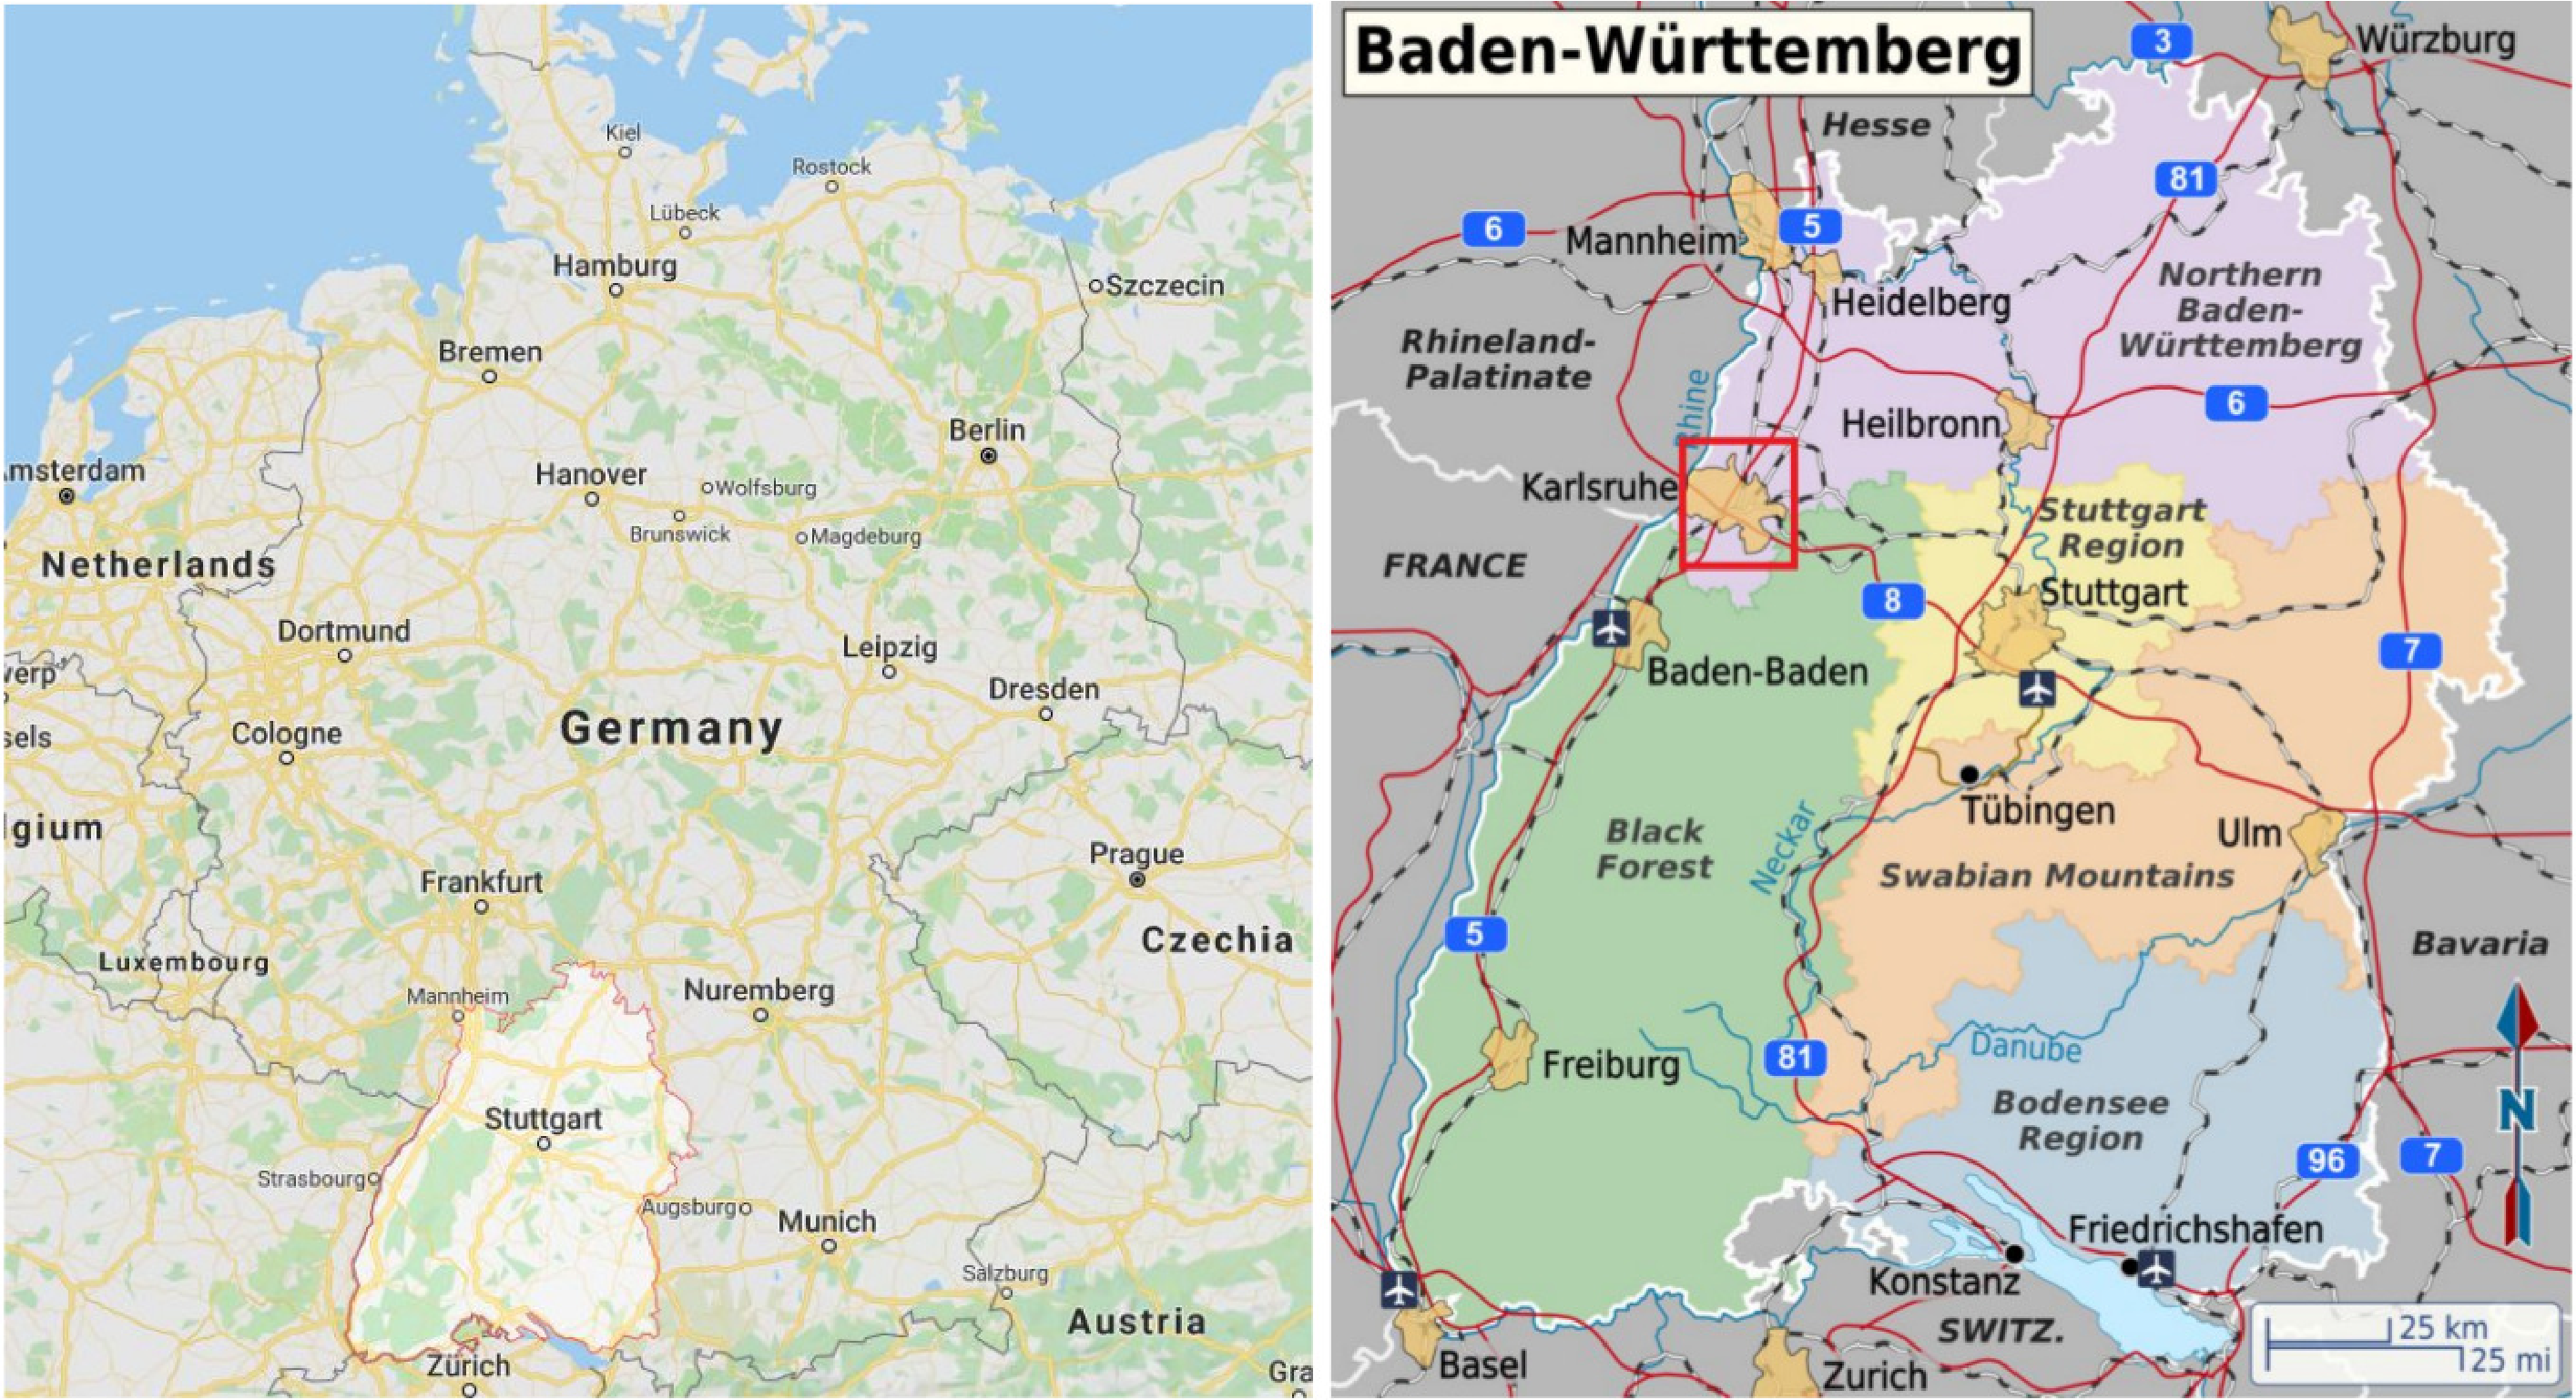
\includegraphics[width=\linewidth]{fig/mapakit.eps}
    \caption{Map of Germany with Baden-Wüttemberg marked (left) \cite{badenmap} and location of Karlsruhe within the state (right) \cite{karlsmap}}
    \label{fig:mapakit}
\end{figure}

Nowadays, KIT is one of the most prestigious technical universities in Germany, specializing on engineering
and science. Figure \ref{fig:kitlogo} shows the current logo of the university. KIT is conformed by a scientific organization
separated by divisions:

\begin{compactitem}
    \item Division I: Biology, Chemistry and Process Engineering.
    \item Division II: Informatics, Economy and Society.
    \item Division III: Mechanical and Electrical Engineering.
    \item Division IV: Natural and Built Environment.
    \item Division V: Physics and Mathematics.
\end{compactitem}

\begin{figure}
    
\includegraphics[width=\linewidth]{fig/kitlogo.eps}
    \caption{Logo of the Karlsruher Institut für Technologie \cite{kitlogo}}
    \label{fig:kitlogo}
\end{figure}

These divisions are constituted by departments destined to investigational work, innovation and teaching.
Each department has institutes responsible for university education. Aside from the institutes, there are
KIT centers, on which topics related to investigation and innovation go beyond the divisions, supporting
an interdisciplinary cooperation \cite{kitorg}. 


The Department of Informatics is one of the first to be established on Germany. This department is formed
by different institutes focused on teaching and investigation of topics associated with informatics. As
part of the Department of Informations the CES comes as a center of investigation on aspects related
with the design of embedded systems, from the reliability of electrical circuits to the management of
electrical power on systems with multiple and many cores.

\subsection{Knowledge area}

The project is developed within the technical area of approximate computing, which is part of the areas
of interest of computer engineering. Approximate computing looks to relax the numerical equivalence 
between the specification and implementation of such applications, approximate computing promises significant 
energy-efficiency improvements and has gained significant traction over the past few years \cite{surveyqu}. Within
appromate computing, the project focuses on the utilization of \intelOCL to develop approximate hardware
kernels and their application on CNNs, highlighting the effect of these kernels on the improvement in 
performance and reduction on energy consumption in comparison to exact kernels.

Furthermore, OpenCL is a tool that allows to define procedures on heterogeneous platformes through the 
use of a high-level programming language. The knowledge on hardware changes via the use of a software 
description is necessary to develop the project.

\subsection{Similar works}

In the area of implementing neural networks on FPGA using OpenCL, notable previous works are:
\begin{itemize}
    \item Suda et al. introduce a complete OpenCL-based accelerator design for CNNs based on
    matrix multiplication. They also explain algorithms to apply convolution by rearranging
    the components of the input image. This work is an exact CNN that could be used as a base
    for the current project. \cite{suda}
    \item Wang et al. propose a CNN implementation on FPGA specifically taking advantage of 
    the ability to allow communication between layers through data channels \cite{pipecnn}.
    \item Zhang and Li present a model to analyse the resource usage on an FPGA, as well as
    implementing their own accelerator based on OpenCL \cite{zhangcnn}.
\end{itemize}

Regarding the use of approximate computing for CNNs, we can find the following related works:
\begin{itemize}
    \item Moons et al. show that using approximations on popular CNNs can increase the energy
    efficiency of the accelerators and show some of the techniques that can be applied to other
    CNNs \cite{moons}.
    \item Kamel et al. compile a lot of techniques that can be used on CNNs and some other 
    information regarding the application of CNNs on FPGAs \cite{kamel}.
\end{itemize}

Also, there is the work done by D. Spies [reference missing as the thesis has not been published yet]
on which some CNN frameworks were implemented for low-power FPGAs, reducing the need for high-end
FPGAs and allowing for further research on the area.

\section{Problem statement}

\subsection{Problem context}

In the last years, discussions on the physical (and economical) limits of the very large scale integration 
of transistors have surfaced \cite{aftermoore}\cite{moorelawlimit}, where statements like Moore's Law exert pressure the big chip manufaturers.
Gordon Moore himself has assured that this trend cannot be maintained for a long time \cite{mooredead}. This leads to the
search of new paradigms or techniques that allow to sustatin the high requirements on performance and 
energy consumption of applications in the technological world, where a need to process even higher amounts
of data is increasing. Some solutions to this increasing demand have appeared, such as multicore computers,
multithreading architectures, large scale computers, GPU processing and more.

Despite these solutions, there exist other problems that cannot be solved just by improving on the architecture
of the processor. Some of these problems are:

\begin{compactitem}
    \item The memory wall: Wulf and McKee\cite{memorywall} describe an inminent problem on which the superior speed increase
    of the processors is a lot higher that the improvement on memory technologies. This requires solutions that
    try to reduce the amount of memory accesses.
    \item The utilization wall: Taylor et al.\cite{utilizationwall} noticed a phenomenom that appears due to the increase on the amount
    of transistors per unit of area in a chip. The problem is related to an exponential reduction of the usable
    percentage of the chip depending on the scale of integration of the transistors.
    \item Problems with thermal dissipation: with the increase of frequency of the microprocessors, the level of 
    heat disipation has increased, forcing a reduction on the operational voltage. Some solutions have been proposed
    to this problem, like the utilization of multicore processorss with cores that deactivate themselves to reduce
    the workload \cite{whitepaper}.
\end{compactitem}

Due to these problems and the increasing existence of error-resilient applications (e.g. \cite{errortolerant}) paradigms such as
approximate computing have appeared. This paradigm tries to eliminate, or reduce, the need for precision
during processing with the goal of obtaining gains in energy efficiency and processing speed.

Furthermore, one area of interest withing the error-resilient application world is machine learning.
The goal of this area is to allow a computational system to execute tasks without the need for a prior
specific programming and, in some cases, using previous results as feedback to improve the execution.
Algorithms used in machine learning look to build mathematical models based on "training" data to perform
tasks without explicit programming \cite{patternrecogbook}. Due to their nature, machine learning applications do not present
an exact response inmediately, or even never, instead they require multiple feedback cycles to achieve
the expected response. This means that approximate computing is a potential paradigm to work with this
type of applications \cite{approximatecomp}.

\subsection{Justification of the problem}

Approximate computing is an area that is till in the upswign. There are diverse investigations and designs
that look to take advantage of the existence of error-tolerant applications. However, it is necessary to
continue advancing the paradigm and develop new techniques in order to observe its contributions in daily
life. The importance of this paradigm resides on the fact that it does not depend on the current state
of the technology to bring forth energetic and performance improvements.

The use of FPGA in the area of approximate computing is still under explored. At the same time, machine
learning applications are of great interest to a lot of fields. An improvement on current machine learning
implementations through the combination of both areas would generate new opportunities and solutions
with low energectic consumption and high adapdability levels. Following this thought, the project is
important due to the following:

\begin{compactitem}
    \item It allows to advance the investigation on the area of approximate hardware definition
    using popular tools such as OpenCL, which could be used as the basis for future investigations
    with FPGA based applications.
    \item The use of a popular and easy to use tool could speed up the generation of results in a
    less explored area, such as FPGA implemented neural networks.
    \item The project generates new tools easily adaptable to machine learning applications based
    on neural networks. These tools can be individual kernels or sets of customizable kernels. 
    \item New investigations on error tolerant applications and approximate computing can easily 
    make use of the findings of this project.
\end{compactitem}


\subsection{Problem definition}

Machine learning applications are based on different methods used to obtain results.
One of the most used techniques are called neural networks, with the objective of imitating the work
done by the human brain to obtain similar results. Furthermore, there is a branch of neural networks
called deep learning. It consists in the increase of the amount of processing layer in order to obtain
a bigger amount of details from an input of data \cite{deeplearningoverview}. Layers are represented by nodes (neurons)
that process data from the input. This processing requires a high level of computation, but its
results are mostly approximations. CNNs are part of the deep learning neural network implementations, with most
of its usage focused on analyzing input images.

Now, FPGAs are devices that have been recently the object of investigations with the objective of accelerating
the current processing being done. The interest in using FPGAs for high amounts of computation comes from
the limitation of general use CPUs, which do not offer enough processing power (multiple operations with 
high level of complexity at the same time); and GPUs that, even with the capability of processing high
amounts of data at the same time, are not specialized enough or even customizable to perform specific tasks.
The use of a device that can be programmed at the hardware level for specific tasks (in this case, neural networks)
offers possibilities on processing speed and energy efficiency that surpass GPUs \cite{surveyfpgann}.

The current project emerges with the objective of contributing to the ongoing investigation efforts
in the area of FPGAs for machine learning applications through approximate hardware definition.
Each neuron in a neural network is represented as a "hardware kernel" that gets defined the 
calculations and processes that it needs to do on the input data to analyze it.
Through the use of software tools like OpenCL, it is possible to define kernels that perform
machine learning tasks. So, combining all these areas and tools, an improvement on performance and
energy consumption must me possible to supply the global demand of processing.

\section{Objectives}

\subsection{Main objective}

Design an approximate hardware implementation of CNNs through the 
use of \intelOCL.

\subsection{Specific objectives}

\begin{compactitem}
    \item Describe the viable changes on the OpenCL tool for approximate hardware generation on FPGA.
    \item Create aproximate and reusable hardware kernels for CNNs using OpenCL.
    \item Determine the error-tolerance level of CNNs when using approximate kernels instead of exact kernels.
    \item Ascertain the reduccion of computational resources when using approximate kernels compared to the use of traditional exact kernels.
\end{compactitem}

\section{Scope, deliverables and limitations}

\subsection{Scope}

The project's end goal is designing, developing and implementing approximate hardware kernels on FPGA.
These kernels represent each of the layers of a CNN and will allow for an image processing algorithm to be
performed on them. The end result must be more energy efficient and provide better performance over existing
implementations of CNNs.

The project is subdivided in the following stages:

\subsubsection{Theoretical investigation}

A first step is to investigate on the following topics:

\begin{itemize}
    \item Convolutional neural networks.
    \item OpenCL and hardware definition.
    \item Approximate computing on neural networks.
    \item CNN implementation on FPGAs.
\end{itemize}

This will provide the necessary information to use OpenCL to implement CNNs on FPGA.
Futhermore, this information can also be used to generate mathematical models to measure the error
and precision of the generated CNNs, be them exact of approximate, as well as the comparison between
both implementations.

\subsubsection{Exact CNN implementation on FPGA}

An exact CNN implementation must be developed in order to have a baseline in order
to develop the approximate kernels. This exact CNN implementation is also used to
compare results in order to evidence the performance and energy efficiency improvements.
Finally, the approximate CNN implementation must be a modification of the exact model.

\subsubsection{Approximate CNN implementation on FPGA}

This implementation must be completely based of the exact CNN implementation and will 
reflect the OpenCL changes that allow for a different hardware definition, one that is 
approximate and adds errors in the processing of the input data. Also, the approximate
implementation must have a set maximum error, which should be measurable and used
in the mathematical models.

\subsubsection{Comparison and mathematical modeling}

Using the results of both the exact and approximate implementation, a mathematical model
should be created that reflects the changes in the error between the exact and
approximate implementation of the CNN. This model will indicate which parameters could
be changed in the approximate implementation in order to reduce or increase the error, as well
as the repercussions in performance and energy consumption.

\subsection{Deliverables}

\begin{enumerate}
    \item Theoretical investigation
        \begin{enumerate}
            \item Compilation report of the use of neural networks on FPGA: this report will contain
            relevant information to be used in the rest of the project and will enable the decision
            making in regards to neural networks on FPGA. 
            \item Progress report with the viable modifications: report with the modification possibilities
            with OpenCL and that affect the hardware definition on FPGA.
        \end{enumerate}
    \item Design stage
        \begin{enumerate}
            \item Documentation on how to approximate neural networks: contains the necessary information
            on the principles of approximate computing that are applicable on neural networks, specifically
            for CNNs. It should contain mathematical models that can be compared against the results
            of the project.
            \item Design of the error calculation model: contains the mathematical formulations that allow
            to create a precise calculation of the results that will be obtained so they can be compared
            with the gain in performance.
        \end{enumerate}
    \item Code development
        \begin{enumerate}
            \item Source code: source code of the OpenCL application and any other code necessary to
            compile, execute and test the kernels.
            \item Exact kernels: source code of the exact kernels used as a base line for the approximate kernels.
            \item Approximate kernels: source code of the approximate hardware kernels that will be used
            on the testing phase.
        \end{enumerate}
    \item Testing stage
        \begin{enumerate}
            \item Results of the exact tests: measurements of performance, precision and energy consumption while
            testing the exact kernels.
            \item Results of the approximate tests: measurements of performance, precision and energy consumption while
            testing the approximate kernels.
            \item Results documentation: comparison of the results between exact and approximate tests.
        \end{enumerate}
    \item Project administration
        \begin{enumerate}
            \item Design document: contains the design of every tool developed during the project.
            \item Meeting minutes: contains all information obtained in the progress and validation
            meetings.
            \item Final report: final report of the project with all relevant information that was
            generated during its course.
        \end{enumerate}
    
\end{enumerate}

\subsection{Limitations}

LIM-01: the student must movilize to Germany in order to have less conflicts with the project supervisor.
Because of the lack of a visa, the time in the european country is limited to 3 months. 
 
LIM-02:​ the student's budget is only 1000 euros during the stay in Germany.

LIM-03: the student must comply with the regulations and limitations of the KIT in regards to international
students.

LIM-04: no face to face meetings are possible with the advisor teacher due to the geographical location of 
the student during the project. Every meeting and communication must be done via the internet.

LIM-05: the project is based on a master thesis developed more than a year before the start of the current
project. As such, compiling and executing the prior project limits the progress on the current project.

% \subsection{Risks}

% RIE-01: ​ Recibir un rechazo de la solicitud de la visa. El proceso de solicitud de visa ya fue iniciado, pero
% existen diversos factores que pueden hacer que la visa sea rechazada y que están fuera del control del
% estudiante.
% - Probabilidad: media. Existe un antecedente de la extensión de solicitud de visa por parte de otro
% estudiante que realizó el mismo viaje hacia Alemania.
% - Impacto: medio. El no tener visa significa que el tiempo de estadía en Alemania se reduce a 3
% meses. El tiempo no se reduce demasiado, pero eso añade una presión extra al estudiante y
% reduce el tiempo efectivo de desarrollo del proyecto.
% - Acciones mitigadoras: se va a iniciar el proyecto con la sección de investigación un tiempo antes
% del viaje hacia Alemania para reducir el impacto de una reducción del tiempo de estadía.

% RIE-02: No conseguir un lugar de residencia para la fecha de llegada a Alemania. Los procesos de
% obtención de residencia en Alemania contienen diversos pasos, entre ellos una entrevista personal que
% supone una mayor dificultad para obtener un lugar de estadía.
% - Probabilidad: baja. A pesar de que cada lugar tiene diferentes procesos, existen muchas
% opciones de estadía y el precio de alquiler no supone un riesgo para el proyecto. Además,
% existen opciones para alojarse mientras se busca una estadía permanente.
% - Impacto: bajo. De no encontrar un hospedaje para la fecha de llegada, el estudiante deberá
% disponer de tiempo de desarrollo del proyecto para conseguir el hospedaje.
% - Acciones mitigadoras: el estudiante debe agotar todas las opciones existentes de hospedaje
% meses antes del viaje a Alemania para aumentar las posibilidades de conseguir alojamiento.
            
% RIE-03: El estudiante deberá obtener un vuelo que se adapte a las necesidades de fecha de inicio de las
% tareas en Alemania y a las limitaciones de tiempo impuestas por la visa (o falta de ella). Debido a que los
% vuelos suponen un complejo sistema de escalas y destinos, existe un riesgo de obtener un vuelo que
% llegue a Alemania en una fecha posterior a la prevista.
% - Probabilidad: baja. Existen múltiples opciones para conseguir vuelos que se adapten a las
% diferentes necesidades de las personas.
% - Impacto: baja. El proyecto se podría retrasar varios días.
% - Acciones mitigadoras: se debe obtener un vuelo que satisfaga las necesidades del estudiante
% con anticipación y estar atento a nuevas opciones.

% RIE-04: La universidad KIT permite a todo estudiante admitido ser registrado en ella. Esto ofrece
% beneficios específicos para estudiantes matriculados en universidades alemanas, como descuentos en
% transporte público. El riesgo está en que el registro no pueda ser completado.
% - Probabilidad: baja. El estudiante ya fue admitido en la universidad y el cumplir con todos los
% requisitos reduce la posibilidad de que el registro sea rechazado.
% - Impacto: baja. El no ser registrado podría provocar un aumento en los gastos financieros del
% estudiante,. Sin embargo, esto no supone mayor inconveniente.-
% Acciones mitigadoras: el estudiante ha ahorrado dinero extra en caso de necesitar realizar
% gastos mayores de los esperados.

% RIE-05: El proyecto depende de que la herramienta de software permita modificaciones adecuadas para
% la definición de hardware aproximado en FPGA. Un riesgo del proyecto es que la herramienta no
% permita realizar definición de hardware no exacto.
% - Probabilidad: media. La herramienta a utilizar es Intel® FPGA SDK for OpenCLTM. Este es un
% framework de código-cerrado.
% - Impacto: medio. De no ser capaz de utilizar OpenCL para desarrollar el proyecto, se deberá
% acudir a otras opciones, esto retrasaría el proyecto.
% - Acciones mitigadoras: el estudiante deberá buscar otras opciones antes de iniciar el proyecto
% para evitar un bloqueo en el proyecto.

% RIE-06: De ser capaz de realizar modificaciones en la definición de hardware obtenida por parte de la
% herramienta, existe el riesgo de que estas modificaciones no sean suficientes para obtener hardware
% aproximado para kernels de redes neuronales.
% - Probabilidad: media. Esta es una de las mayores incertidumbres del proyecto y parte de los
% resultados de la investigación teórica.
% - Impacto: alto. El no ser capaz de realizar modificaciones para obtener hardware aproximado
% significa un replanteamiento por completo del proyecto.
% - Acciones mitigadoras: la primera tarea que debe realizar el estudiante es investigar las
% diferentes modificaciones que se deben realizar para reducir la incertidumbre del proyecto.

% RIE-07: Con la suposición de que es posible aproximar el hardware generado por la herramienta de
% software, aparece el riesgo de que la aproximación realizada en redes neuronales no permita tener un
% error suficientemente aceptable en los resultados prácticos de los algoritmos de aprendizaje.
% - Probabilidad: baja. Existen diversos estudios que tratan el tema de aproximación de redes
% neuronales.
% - Impacto: medio. Aunque no se obtenga un resultado positivo en algoritmos de aprendizaje, el
% proyecto puede tener resultados que permitan potenciar otras investigaciones.
% - Acciones mitigadoras: el estudiante deberá mantenerse informado con respecto a las
% posibilidades de mejora en redes neuronales así como los niveles de error que pueden ser
% considerados como aceptables.

%%% Local Variables: 
%%% mode: latex
%%% TeX-master: "main"
%%% End: 

  \chapter{Theoretical framework}
\label{ch:marco}

\section{Convolutional neural networks}

Here, I talk about CNNs.

Start by defining what a neural network is, what they are used for.

Specify that I am working with Convolutional ones, part of Deep Learning.
Explain what is convolution and the main CNNs frameworks (tensor, caffe, alex).

Major uses and examples of uses.

%------------------------

A standard neural network consists of many simple, connected processors called neurons,
each producing a sequence of real-valued activations. Input neurons get activated through 
sensors perceiving the environment, other neurons get activated through weighted connections from previously
active neurons.
Learning is about finding specific weights that make the network exhibit desired behavior,
such as driving a car. Depending on the problem and how the neurons are connected, such behavior
may require long causal chains of computational stages, where each stage transforms 
the aggregate activation of the network. Deep Learning is an area of machine learning that tries to
replicate this behavior by increasing the number of stages \cite{schmidhuber2015deep}.



CNNs are part of deep learning, a type of neural networks based on the 
visual system of mammals \cite{fukushima1980neocognitron}\cite{hubel1968receptive}.
A CNN is usually comprised of three types of layers: convolution, pooling and 
fully-connected \cite{karpathy2016cs231n}. A CNN differs from a regular neural network
by the amount of connected layers and configurations, figure 

southwest of Germany. Figure \ref{fig:mapakit} shows a map with the location of Baden-Württemberg inside the european
country and the location of Karlsruhe inside the aforementioned state.

\begin{figure}
    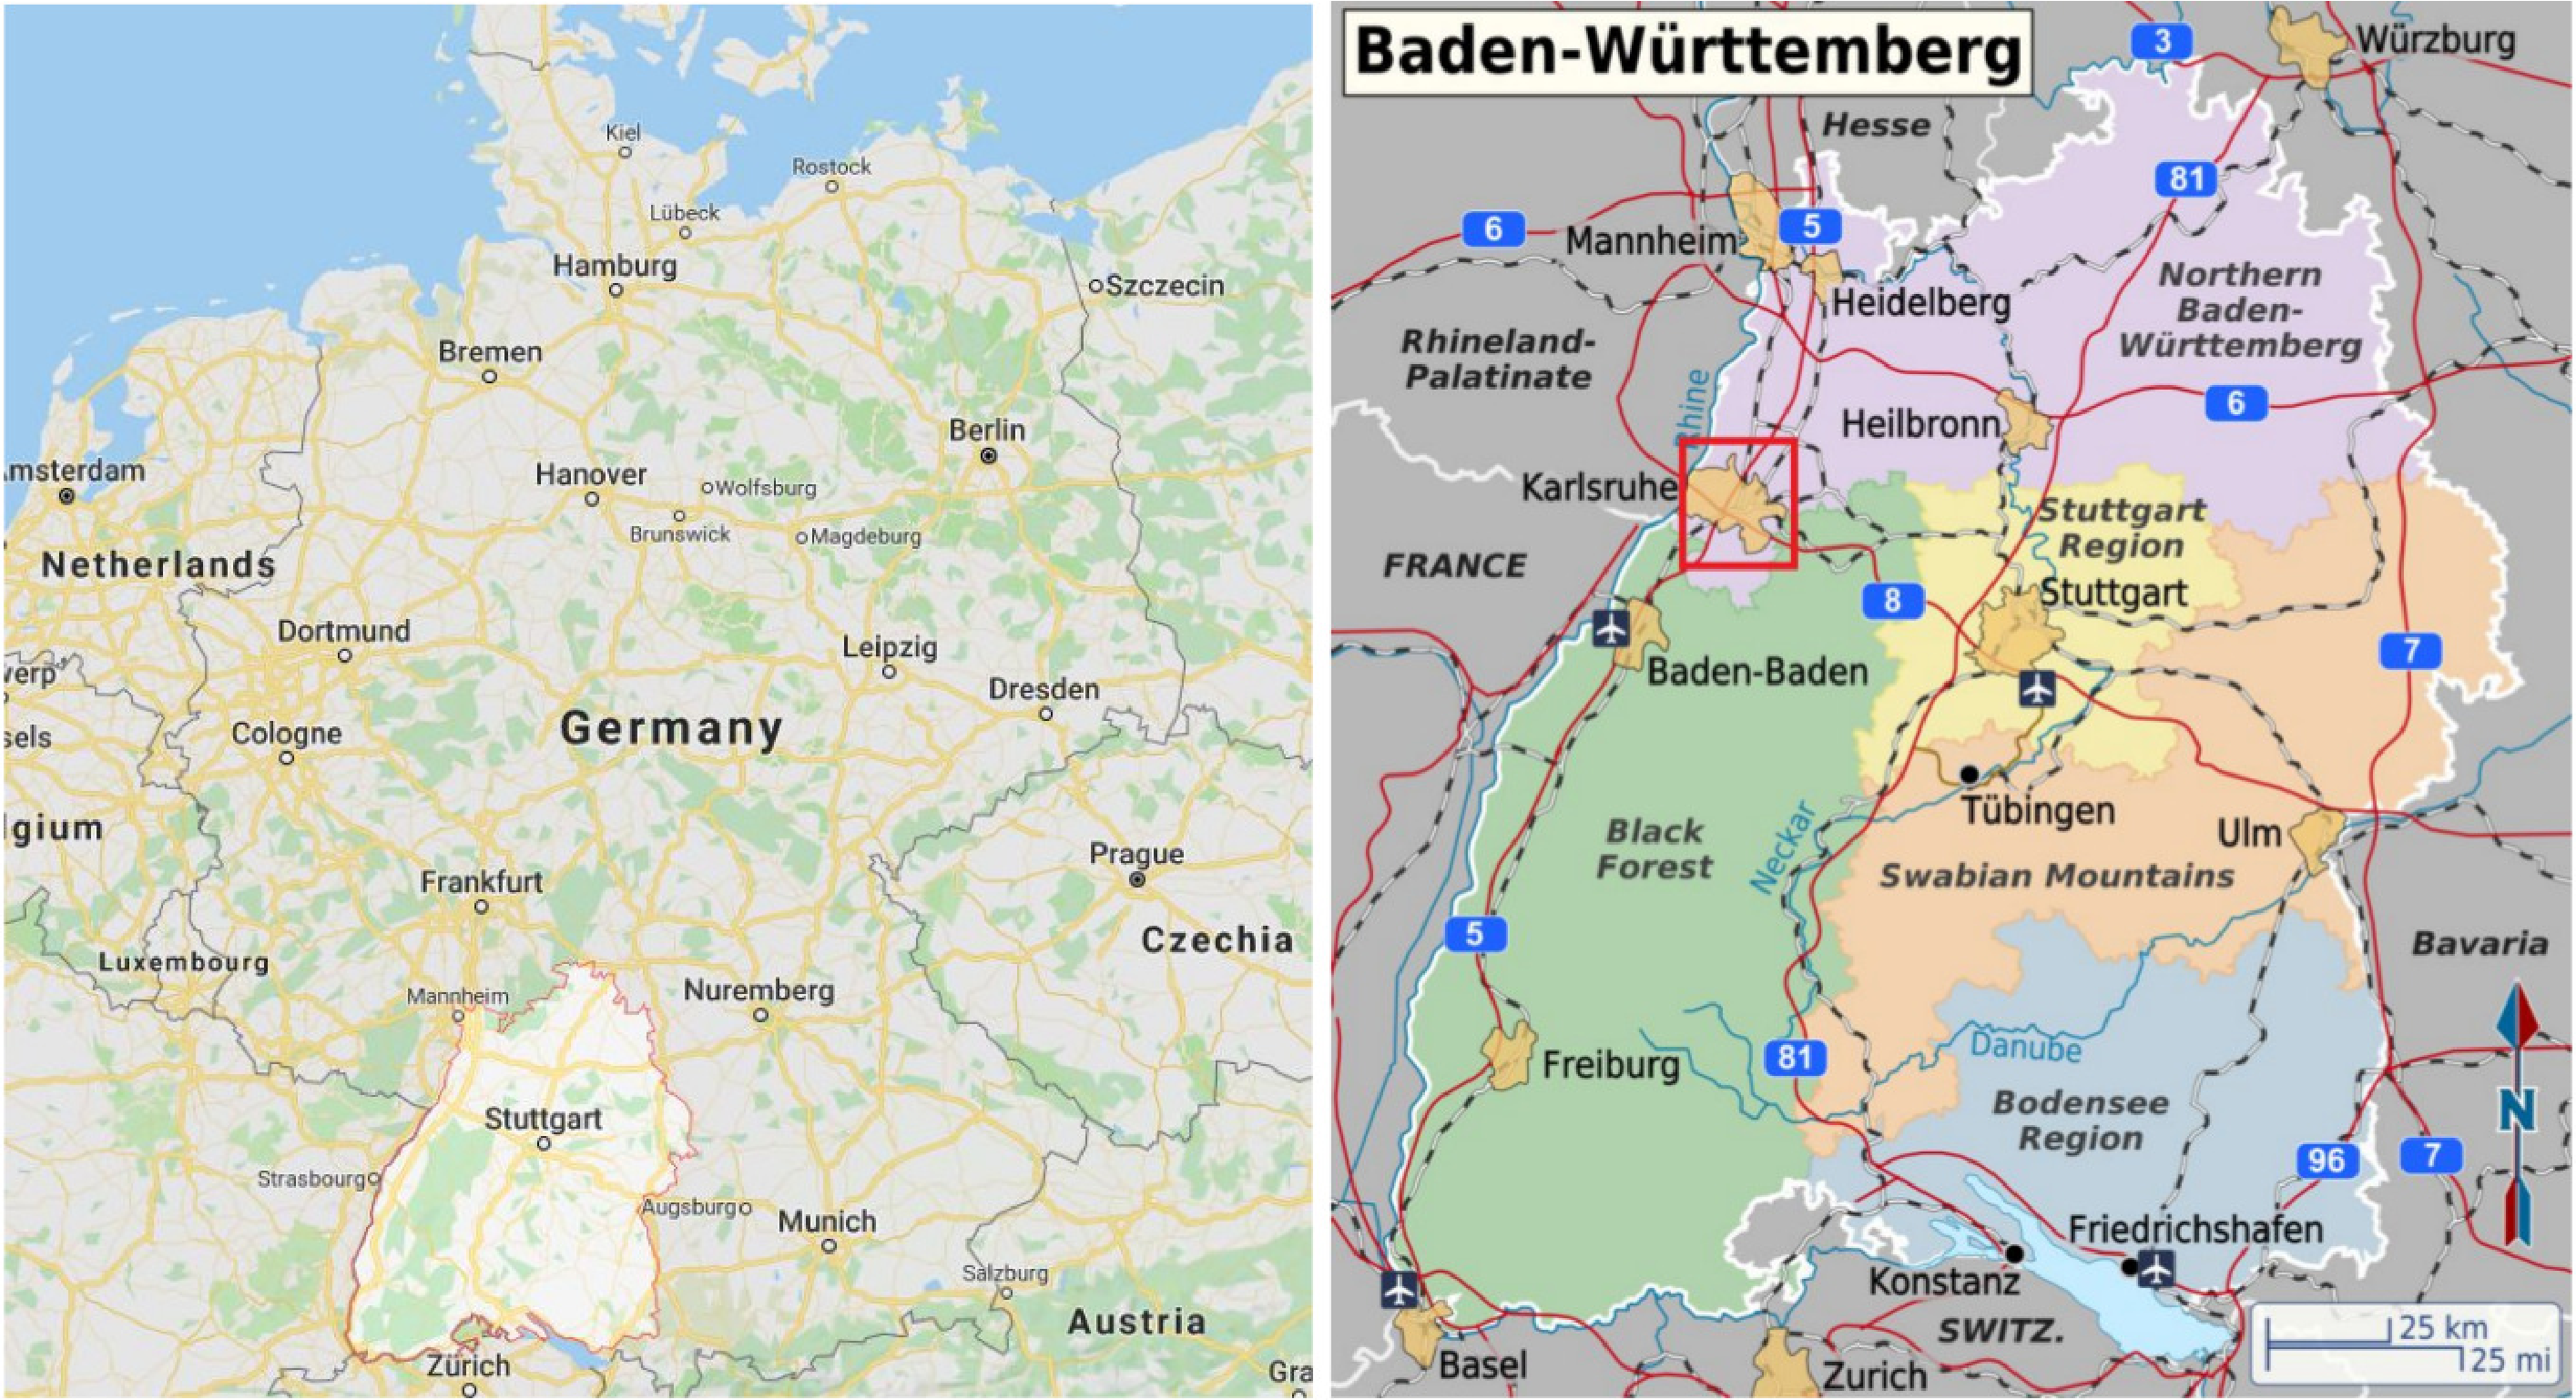
\includegraphics[width=\linewidth]{fig/mapakit.eps}
    \caption{Map of Germany with Baden-Wüttemberg marked (left) \cite{badenmap} and location of Karlsruhe within the state (right) \cite{karlsmap}}
    \label{fig:cnn}
\end{figure}

The use of heterogeneous devices, from general-purpose GPUs to FPGAS, to execute 
machine learning algorithms and neural networks
is of big interest in the current world and there are current efforts to bring
all types of devices together \cite{abadi2016tensorflow}.



A general example for a deep neural network is
shown in figure 2.1: The first, left-most layer is the input layer which is connected to the
first of several hidden layers. In this example, each hidden layer is again connected to one
successor layer until reaching the final output layer on the far-right side. Consequently,
each layer is responsible for reading multiple input values, applying an operation on them
and providing the resulting value to the next layer. For example, during such operations,
each input value is multiplied with a corresponding weight value which is stored as a layer
parameter, after which the results are accumulated (multiply-accumulate operation). In fig-
ure 2.1, this is illustrated as lines of different colors and saturation, representing input/output
values of lower and higher magnitude. These weight values of neural networks are typically
learned through algorithms to optimize the network functionality for its designated task.

Additionally, because operations in neural network layers are usually linear combinations, a
non-linearity called activation function is added after each layer to allow for computation of
non-trivial problems. Without this non-linear separation of layers, they could be combined
and reduced to a system of linear functions in a single layer. In such networks, it is not
possible to implement complex functions like the XOR (exclusive or) logical function [11].
In recent years, different kinds of neural networks have been proposed, involving different
types of layers and fields of application in general. For visual applications such as image
classification and face detection, the class of convolutional neural networks (CNNs) has
shown superior results and is very prominent today [4, 5, 6]. Based on the research of
Hubel and Wiesel [12] on the visual cortex, CNNs are created to emulate the processing
of images in the brain. As with the general deep neural networks described above, CNNs
consist of several hidden layers surrounded by one input and one output layer. Starting with
the input image, data is passed to the input layer and processed by each layer of the network.

Each layer receives input data from its predecessor, applies the corresponding operations
and delivers output to its successor. Ultimately, the output layer contains the classification
result for the input image. Typically, each layer is either a convolutional, a pooling or an
inner product (fully connected) layer. However, many methods from literature introduce
novel techniques and layer types such as local response normalization (LRN) to improve the
accuracy and performance of their proposed network model [4]. The AlexNet CNN model
is shown in figure 2.2 and illustrates the application of multiple convolution layers, paired
with max-pooling and inner product (dense) layers. The most common CNN layer types are
described in detail in the following paragraphs.

%-----

\section{Approximate computing}

What is approximate computing. What is the problem it is solving and
how it solves it. Some of the layers for approximate computing.

Approximate computing on hardware definition and algorithms.

Approximate computing on FPGAs.

Approximate computing on CNNs.

\section{\intelOCLnos}

Talk about OpenCL and its main objective. Talk about kernels.

Talk about the specific SDK created by Altera to be used on FPGAs.

Some facts about the precision of it vs writing manual Verilog.

How OpenCL has been used to describe CNNs on FPGA. (Suda, Pipe, other)

Why OpenCL on FPGA vs using a CPU or GPU.


\section{Descripción}

Toda tesis hace referencia a trabajos previos en el área y trabajos afines que
están directamente relacionados con lo planteado en el tesis.

Además, en el marco teórico debe aparecer la información absolutamente
necesaria para comprender la solución, y por eso es recomendable escribir
primero la solución (el siguiente capítulo), para ir anotando qué debe ser
explicado en el marco teórico.

\section{Generalidades}

Se recomienda revisar las guías de publicación de la \nt{IEEE} en
\url{http://www.ieee.org/publications_standards/publications/authors/authors_journals.html},
donde puede encontrar cómo hacer referencias bibliográficas correctamente, cómo
citar ecuaciones, tablas y figuras, etc.  

\subsection{Redacción}

La \nt{redacción} en todo el documento debe seguir un estilo científico
objetivo. Esto implica que se redacta de modo impersonal, sin utilizar primeras
personas del singular o del plural, y se evita el uso de cualquier tipo de
calificativo, sustituyéndolos siempre por datos concretos, vinculados a
referencias bibliográficas o datos experimentales. Los comparativos también
deben concretarse a hechos y datos, y nunca dejarse ``en el aire''. Por la
naturaleza de la tesis, el tiempo verbal es usualmente presente, no perdiendo
nunca de vista que se está explicando ``cómo hacer algo'', en vez de ``qué se
hizo''.

Las \nt{frases} deben ser cortas, y debe evitarse que el lector tenga que saltar
constantemente entre partes de la tesis, lo que implica una exposición lineal
clara, donde lo que se necesita ya ha sido explicado antes. Deben evitarse
redundancias y por tanto cada concepto se exponen en un único lugar.

Todo aspecto circunstancial es irrelevante para la tesis, es decir, si se ha
desarrollado en el laboratorio $X$, o en el curso $Y$, con el profesor $Z$, o
en la empresa $W$, el nombre de funciones o clases en su código, etc., es
información irrelevante para reproducir el experimento, y por lo tanto sobra.
%
Esa información puede incluirse en uno de los anexos.


\subsubsection{Numeración del documento}

La primera página de la tesis es la correspondiente a la introducción,
así que ésta debe ser la página 1. Desde la introducción, hasta antes
de la bibliografía, las unidades son ``Capítulos''. La bibliografía y
anexos no se consideran capítulos, así que ya no continúan con la
misma numeración de los capítulos (la paginación sí continua). Los
índices, notación, glosario, etc.\ se numeran con números romanos en
versalitas ({\textsc{I}, \textsc{II}, \textsc{III}, \textsc{IV},
  \textsc{V}, \textsc{VI}}$\ldots$) y antes del índice (portada,
resúmenes, agradecimientos, hoja de evaluadores, etc.) las páginas no
llevan numeración.

Esta plantilla LaTeX ya se ocupa de todo lo anterior.

\subsection{Ecuaciones}

Para citar \nt{ecuaciones} se utilizan paréntesis redondos, y no es
necesario emplear explícitamente la palabra ``ecuación''. Por ejemplo
``Introduciendo en (4.2) los resultados de (3.3) y (3.7) se obtiene
...''. La ecuación es parte del flujo de texto y no un objeto
flotante, así que no pueden emplearse como figuras. Cuando se requiere
la ecuación, allí se inserta.

Es incorrecto redactar de la siguiente forma: \explain{MAL}

\textsl{La operación del transistor sin tomar en cuenta el efecto Early está
  dada por (\ref{eq:ej1}), donde el parámetro $\kappa$ está dado por
  (\ref{eq:ej2}).}

\begin{equation} \label{eq:ej1}
  I_{DS}
  =
  I_{n0} \frac{W}{L}e^{\kappa \frac{V_{GB}}{v_t}}
  \left[
    e^{-\frac{V_{SB}}{v_t}}
    -
    e^{-\frac{V_{DB}}{v_t}}
  \right]
\end{equation}

\begin{equation} \label{eq:ej2}
  \kappa = \frac{C_{ox}}{C_{ox}+C_{dep}}
\end{equation}

Lo anterior es incorrecto porque obliga al lector a estar buscando ecuaciones,
que pueden mostrarse directamente.  La única referenciación permitida es hacia
atrás.

La forma correcta de redactar lo anterior es: \chk{BIEN}

\textsl{La operación del transistor sin tomar en cuenta el efecto Early está
  dada por}
\begin{equation} \label{eq:ej3}
  I_{DS}
  =
  I_{n0} \frac{W}{L}e^{\kappa \frac{V_{GB}}{v_t}}
  \left[
    e^{-\frac{V_{SB}}{v_t}}
    -
    e^{-\frac{V_{DB}}{v_t}}
  \right]
\end{equation}
\textsl{donde el parámetro $\kappa$ es}
\begin{equation} \label{eq:ej4}
  \kappa = \frac{C_{ox}}{C_{ox}+C_{dep}}
\end{equation}

Así el flujo del texto guía al lector por las ecuaciones sin mayor esfuerzo.

Es recomendable numerar \emph{todas} las ecuaciones, de modo que en la revisión
del documento, o en futuras referencias a su documento de tesis todas las
ecuaciones puedan ser citadas sin requerir describir textualmente a cuál
ecuación se está haciendo referencia.

Es preferible utilizar coma decimal en vez de punto decimal, debido a
que es el estándar internacional.  El Diccionario panhispánico de
dudas aclara que se acepta el punto como separador decimal, pero eso
no quiere decir que sea preferible.  Esta plantilla ya incorpora el
uso del paquete de \LaTeX\ \code{icomma}, que se encarga de realizar
el espaciado correcto de la coma.  Cuando utilice coma como signo de
puntuación, deje un espacio posterior, para asegurarse de que
\code{icomma} no lo tome como separador decimal.

\begin{equation}
  \label{eq:normrnd}
  h(x)=\norm{\rand()-0,5}^2_2
\end{equation}

\subsection{Figuras}

Para el almacenamiento de imágenes existen dos tipos de formato: las imágenes
raster y las imágenes vectoriales.\index{imagen!raster}

\subsubsection{Imágenes raster}

Las imágenes raster son representadas por una rejilla de píxeles, en donde cada
píxel tiene un valor que representa al nivel de gris o el color. La
discretización espacial es ineludible, y la única forma de obtener buena
calidad es empleando tamaños grandes de la imagen que conduzcan a resoluciones
de al menos 300 puntos por pulgada en la impresión, lo que conlleva a archivos
de documentos de varios megabytes. Dentro de los formatos para almacenar
imágenes raster existen algunos con pérdida (como el JPEG) que producen en
imágenes sintéticas, como diagramas, estructuras ruidosas que dan una
apariencia de baja calidad a las figuras. Otros formatos (como PNG, BMP, TIFF o
GIF) no tiene pérdidas de información, pero los algoritmos de compresión no
pueden reducir el tamaño de las imágenes con los mismos factores de reducción
que los formatos con pérdidas. Este tipo de formatos debe utilizarse únicamente
para fotografías o capturas de escenas reales con cámaras digitales.

\subsubsection{Imágenes vectoriales}

\index{imagen!vectorial}
Las imágenes vectoriales \textbf{deben} ser empleadas en todo tipo de
diagrama. En ellas no se almacenan píxeles, sino las estructuras geométricas
que componen la figura como círculos (representado por posicion de su centro y
su radio), rectángulos (representados por sus esquinas), líneas, texto, etc. La
mayoría de programas para elaborar este tipo de diagramas, como Inkscape, XFig,
OpenOffice.org Draw, MS Visio, Adobe Illustrator, etc. proveen varios formatos
vectoriales que pueden ser insertados tanto en LaTeX como en OpenOffice.org
Writer (o MS Word). Los formatos más empleados son los llamados metafiles, que
incluyen al WMF, EMF. En LaTeX se utiliza por lo general EPS. Recientemente se
ha incrementado el soporte al formato SVG.

No debe cometerse el error de generar una imagen vectorial a partir de una
imagen raster, pues una vez realizada la discretización espacial no es posible
reconstruir los elementos geométricos que componen la imagen. Por ello, no
tiene ningún sentido generar un archivo EPS o WMF a partir de una imagen ya
almacenada en BMP, JPG, o PNG, pues lo único que ocurrirá es que se inserta la
figura raster tal cual en la imagen vectorial, sin implicar ninguna ganancia en
la calidad.

Esta plantilla de LaTeX administra la generación de ciertas figuras por usted.
Puede colocar en el directorio \texttt{fig/} archivos EPS, JPG, PNG o GP (de
GNUPlot) y el Makefile se encarga de hacer todas las conversiones necesarias.
En las siguientes subsecciones se describen dos casos adicionales que resultan
útiles para realizar figuras más complejas.

\subsubsection{Figuras tikz}
\index{tikz}

Esta plantilla compila archivos con código en Tikz para generar
figuras.
%
En realidad, lo único que hace el Makefile es compilar con
\code{pdflatex} cualquier archivo \texttt{fig/*.tikz} y dejar el
resultado en el directorio de figuras, aunque el concepto fue pensado
particularmente para generar imágenes vectoriales utilizando las
características de Tikz, biblioteca de LaTeX que es utilizada cada vez
más por su enorme flexibilidad.
%
\begin{figure}[htb]
  \centering
  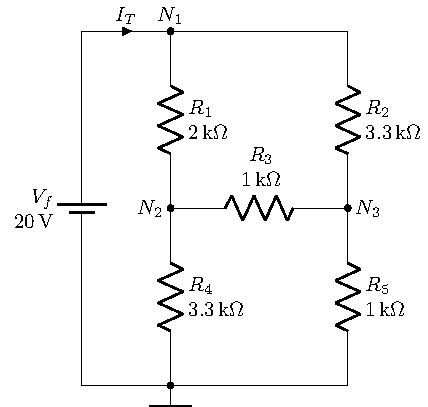
\includegraphics{figtemplate}
  \caption[Ejemplo de figura con tikz]{Ejemplo realizado con
    \texttt{tikz}.  Usted encuentra la plantilla en el directorio de
    figuras bajo el nombre \texttt{fig/figtemplate.tikz}.}
  \label{fig:figtemplate}
\end{figure}

La figura~\ref{fig:figtemplate} muestra un ejemplo que se puede
utilizar como plantilla para generar figuras \texttt{tikz}.  La
plantilla la encuentra en el directorio de figuras y se llama
\code{figtemplate.tikz}.


\subsubsection{Figuras ltxfig/psfrag}

\index{psfrag}\index{ltxfig}
Cuando en el subdirectorio \texttt{fig/} se encuentran dos archivos con el
mismo nombre pero extensiones \texttt{ltxfig} y \texttt{psfrag}, por ejemplo
\texttt{prueba.ltxfig} y \texttt{prueba.psfrag}, entonces el Makefile asume que
usted desea crear una figura a partir del archivo \texttt{prueba.ltxfig},
creado con el programa \texttt{XFig}, sustituyendo los textos ahí presentes con
texto formateado con LaTeX.

La figura~\ref{fig:ltxfig} ha sido creada con este esquema.  Revise los
archivos correspondientes en el directorio de figuras
\texttt{fig/ltxfig\_prototipo.*} para más detalles sobre su uso.

\begin{figure}[htb]
  \centering
  
\includegraphics[width=0.9\textwidth]{ltxfig_prototipo}
  \caption{Ejemplo de imagen ltxfig/psfrag}
  \label{fig:ltxfig}
\end{figure}

\subsubsection{Figuras pstricks}  

\index{pstricks}
Los archivos con extensión \texttt{.pstricks} en el directorio \texttt{fig} se
utilizan para generar cualquier tipo de imágenes según el código que se
contenga.  Es un concepto más general que el anterior.  La
figura~\ref{fig:pstricks} ha sido creada con este esquema.  Puede revisar los
archivos \texttt{prototipo\_gnuplot*} como un ejemplo de su uso, en donde de un
archivo gnuplot (\texttt{\_.gp}) se genera un archivo \texttt{\_.eps}, el cual
es incluido en el archivo \texttt{.pstricks} sustituyendo cadenas de texto por
código LaTeX.

\begin{figure}[htb]
  \centering
  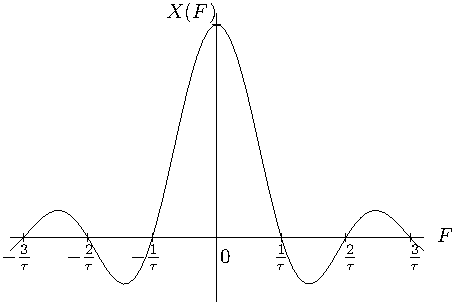
\includegraphics{prototipo_gnuplot}
  \caption{Ejemplo de imagen gnuplot/pstricks}
  \label{fig:pstricks}
\end{figure}



\subsubsection{Entradas en el índice de figuras}

El índice de figuras debe servir para encontrar rápidamente dónde se
encuentra cierta figura.  El pie de la figura, indicado en \LaTeX con
\texttt{caption} puede ser extenso, en especial para indicar detalles
de las figura, y es la entrada por defecto que aparecerá en el índice
de figuras, la cual no debe superar la extensión de una línea y debe
únicamente dar la idea del contenido de la figura para poder ser
encontrada.  Para lograr esto en \LaTeX{} se agrega un parámetro
opcional con el texto del índice de la siguiente forma:
\begin{verbatim}
  \caption[Texto en el índice]{Texto al pie de la figura}
\end{verbatim}

\subsection{Referencias bibliográficas}

\index{referencias}\index{BibTeX}
Todo concepto o idea tomado de otros autores contar con la respectiva
referencia. En redacción técnica de ingeniería rara vez se utiliza la cita
textual, así que es necesario reformular las ideas y conceptos con palabras
propias. En ingeniería electrónica se utilizan los formatos de referencia de la
IEEE o la ACM, que son numéricos, encerrados entre paréntesis cuadrados (por
ejemplo, ``En \cite{Davis1963} se propuso un nuevo algoritmo'', o ``En
\cite{ProakisManolakis1998} los autores proponen tomar las ventajas de los
algorimos presentados en \cite{Oppenheim1998,Roberts2005,Haykin2001} por medio
del método de Newton \cite{Burrus1998} conocido en el área de optimización
lineal.''). La referencia es parte de las frases, así que si la frase termina
con la referencia para indicar la idea, ésta debe estar antes del punto final o
demás signos de puntuación: ``La capacidad de memoria también sigue una Ley
similar a la de Moore \cite{Octave}. Los siguientes son los aspectos a tomar en
cuenta en el diseño del sistema \cite{Lindner2002}:''

Se recomienda utilizar BibTeX para indicar las referencias
bibliográficas.  Actualmente herramientas como Mendeley, Zotero u
otras similares simplifican la administración de las referencias y
pueden exportar al formato BibTeX.

\subsection{Extensión}

\index{extensión}
Una tesis de licenciatura no debe sobrepasar las 120 páginas incluyendo
apéndices y los formalismos desde portada hasta índices.

El cuerpo de la tesis (desde introducción hasta conclusiones) usualmente se
extiende desde 45 páginas hasta no más de 80, dependiendo de la problemática
tratada.

No es necesario reproducir contenidos de otras fuentes: agregue las referencias
a dichas fuentes, y limítese a enunciar lo estrictamente necesario para
comprender sus propuestas de solución.

\section{Sobre esta plantilla \LaTeX}

Esta plantilla \LaTeX pretende simplificar varios pasos en la creación del
documento de tesis.

\subsection{Marcar asuntos pendientes}

La plantilla tiene dos ``\emph{modos}'' de operación: normal y borrador
(\emph{draft}).  En el archivo \texttt{main.tex} a partir de la línea 41 usted
encuentra el código

\begin{verbatim}
%
% DRAFT MODE
%
\newboolean{draftmode}                  % boolean used to control draft-mode
% Ensure that only one of the next two lines is active:
\setboolean{draftmode}{true}            % turn draft mode on
%\setboolean{draftmode}{false}           % turn draft mode off
\end{verbatim}

Con el modo borrador, se activan ciertos comandos y funcionalidades útiles en
el proceso de elaboración de la tesis, pero que deben ser desactivados al
final, antes de entregar la tesis.  Por ejemplo, se activa el pie de página que
dice ``\emph{Borrador: fecha}'', y se activa el índice titulado ``Revisar''.  En dicho índice aparecen las páginas en donde se hayan utilizado alguno de los siguientes comandos:
\begin{compactitem}
\item \verb+\boxcomment{comentario}+ Crea una caja en el margen de página con
  el comentario indicado.
\item \verb+\explain{comentario}+ Crea una caja en el margen de página con
  el comentario indicado, con una flecha hacia la derecha para indicar qué en
  concreto debe ser revisado.
\item \verb+\chk{comentario}+ Crea una caja en el margen con símbolo de
  ``chequeado'' y el comentario indicado.
\item \verb+\TODO{comentario}+ Crea una caja grande de fondo sombreado con el
  comentario indicado.
\end{compactitem}

En este párrafo se\chk{resultado de chk} utilizan algunos de estos comandos
para ilustrar su efecto.  El \verb+\chk+ como puede observar tiene sentido
usarlo para marcar que algo está casi listo.  Por otro lado \explain{explain}
el comando \verb+\explain+ permite marcar algo que requiere ser revisado en
redacción, valores, etc.  El \verb+\boxcomment+\boxcomment{La caja simple}
solo pone una marca al margen.

\TODO{Finalmente el comando \texttt{TODO} coloca esta caja gris.}

Si usted desativa el modo draft, desaparecen todas las marcas
anteriores, y desaparece el índice ``Revisar''.  En éste índice
aparecen todas las páginas en donde se utilizaron estos comandos con
los respectivos comentarios, lo que permite encontrar rápidamente
detalles que usted indicó que debe revisar.

\subsection{Índices}

Como índice se conoce la lista de términos claves con su respectiva
página.  Usualmente aparece al final del documento.  La plantilla
ofrece varios comandos para simplificar el uso estandar del comando de
\LaTeX\ \verb+\index{termino}+ que coloca al término indicado en el
índice.  Con \verb+\nt[indice]{termino}+ (\emph{new term}) usted
indica la entrada principal del término, que aparece en el texto en el
índice, es decir, en el índice aparece lo que indique en vez de
``indice'' y en el texto aparece lo que indique ``termino'';
\verb+\ot{termino}+ agrega una entrada secundaria al término.

  \chapter{Methodology}
\label{ch:metodologia}

The current project is a research on the effect of approximate computing 
techniques to the improvement of performance and energy consumption
on FPGAs. First, the research will be classified based on different perspectives. 
The classification will be
followed by the methods used on creating the CNNs and validating the
changes in execution time, energy consumption and accuracy degradation.

\section{Type of research}

The following classification is based on the different perspectives 
created by \cite{kumar2019research}.

\subsection{Application perspective}

This work is categorized as an applied research. 
The objective is to apply concepts from approximate computing theory
into another field of work or active research such as the study of CNNs on FPGAs.
These concepts will be mixed with other topics from computer architecture
and hardware generation.

\subsection{Objectives perspective}

From an objectives standpoint, this is an exploratory research as it explores the possible 
gains in performance and energy through the use of approximate hardware generation.
The area of approximate computing on FPGAs, specifically for CNN implementations, is currently
underexplored. This research will help grow the field and could enable future research
or applications on using FPGAs to accelerate the field of Machine Learning.

\subsection{Mode of enquiry}

Finally, this is an unstructured research. The objective is to find how different techniques
affect the final measurements and tests in relation to exact kernels. The specific techniques
to be applied are not predetermined. As such, there is no expected accuracy value to be achieved. 
This project tries to 
push performance to the maximum and energy consumption
to the minimum while maintaining an acceptable accuracy, but there is no set number for
any of these values.

\section{Kernel creation}

The research is based on modifications done to an exact CNN implementation on an FPGA. 
The next sections specify the methods used to generate the kernels and apply the 
approximate modifications.

\subsection{Exact kernel generation}

The exact kernel generation will be based on the CaffeNet implementation. This is an AlexNet implementation
with the pooling and normalization layers reversed \cite{donahue2012bvlc}. 

The kernels are implemented using OpenCL on a DE1-SoC board, a hardware board with an on-chip processor and
a Cyclone V FPGA. This board was provided by the university and its use as a CNN accelerator has been tested
previously by other authors \cite{suda}\cite{pipecnn}.
Two codes must be generated, the host code to control the execution of the CNN on
the embedded chip of the board and the device code that will perform the CNN calculations.

The kernels already contain some approximations due to limitations on the FPGA being used, mainly on using
fixed-point values, as it does
not contain enough resources to implement a non-fixed-point implementation of the CaffeNet neural network.

\subsection{Approximate kernel generation}

The approximate kernels will be generated based on modifications done on the exact kernels.
Different techniques will be used to apply these modifications. Any modification must be tested
and different combinations of these modifications must be applied to show the change on accuracy,
performance and resource usage.

The modifications must be applied on varying levels of abstraction, measuring the output on different
layers up to the output of the full CNN.

\section{Validation}

In this section, the validation to be used on the project is explained.

\subsection{Accuracy}

An algorithm based on the formulas found on \cite{googledev} is created using the Python. This algorithm
calculates accuracy of the approximate modifications against a Caffe \cite{jia2014caffe} based AlexNet implementation,
also written in Python.

The training weights to be used for evaluation are the ones found on \cite{donahue2012bvlc}. The original network
was trained using the Image-net Large Scale Visual Recognition Challenge 2012 image set \cite{lsvrc}.
The measurements will be done for top-1 and top-5 accuracy.

\subsection{Resource usage}

For resource usage, the reports generated by \intelOCL will be used in order to get the estimated
resources used in terms of registers, memory, processing units and logic modules.
These reports will be compared against the first implementation on FPGA.
While this does not represent a direct measurement of energy, it can give a small look
into the energy consumption reduction of applying approximate kernels.

\subsection{Performance}

Performance will be measured by a simple difference between the time 
at the end of the image classification and at the start.
This will be compared to the performance of the Caffe implementation 
and the exact implementation with no modifications.
  \chapter{Solution description}

In this chapter the processes, techniques and design decisions made
to get the final results of the project are shown, as well as an analysis
of these results and how they fulfill the objectives of the project.

\section{Solution}

The CNN design and implementation is described in the following sections.
Python is used for the base exact implementation while any approximation is done
using OpenCL.

\subsection{Base CaffeNet implementation}

AlexNet is the winner of the ILSVRC in 2012. Trained using GPUs and based on 3 million training images, it is one
of the best examples that increasing the depth of a NN helps increase its performance and accuracy.

Caffe is a framework created to easily implement, train and execute NNs using Python or C++.
The developers made example models based on popular CNNs, one of which is CaffeNet, a modification of the original
AlexNet configuration with the pooling and normalization layers switched.

Caffe is used to implement an script that uses the training data from \cite{donahue2012bvlc} and executes the network
over 4000 images downloaded from the ImageNet web page. This generates an output that is used as the baseline
for the FPGA implementation and any approximate modification done on the network.

This is a full CPU implementation of CaffeNet using Python. As it is one of the most popular frameworks for CNN
training and implementation, the performance gains and accuracy loses can be measured against it. This project
does not reflect the gains over a GPU implementation due to hardware limitations.

Figure \ref{fig:caffenet} shows the configuration of the CNN. The network has an input matrix of 224{x}224{x}3
and 
contains the following configuration of layers and parameters \cite{reviewalex}:

\begin{enumerate}
    \item Convolutional Layer: 96 kernels of size 11{x}11{x}3
    (stride: 4, pad: 0) with 55{x}55{x}96 feature 
    
    3{x}3 Overlapping Max Pooling (stride: 2)
    27{x}27{x}96 feature maps
    
    Local Response Normalization with 27{x}27{x}96 feature maps
    \item Convolutional Layer: 256 kernels of size 5{x}5{x}48
    (stride: 1, pad: 2) with 27{x}27{x}256 feature maps

    3{x}3 Overlapping Max Pooling (stride: 2) with 13{x}13{x}256 feature maps
    
    Local Response Normalization with 13{x}13{x}256 feature maps
    \item Convolutional Layer: 384 kernels of size 3{x}3{x}256
    (stride: 1, pad: 1)
    with 13{x}13{x}384 feature maps
    \item Convolutional Layer: 384 kernels of size 3{x}3{x}192
    (stride: 1, pad: 1)
    with 13{x}13{x}384 feature maps
    \item Convolutional Layer: 256 kernels of size 3{x}3{x}192
    (stride: 1, pad: 1)
    with 13{x}13{x}256 feature maps
    
    3{x}3 Overlapping Max Pooling (stride: 2)
    with 6{x}6{x}256 feature maps
    \item Fully Connected (Dense) Layer of
    4096 neurons
    \item Fully Connected (Dense) Layer of
    4096 neurons
    \item Fully Connected (Dense) Layer of 1000 neurons (for each of the 1000 classes)
\end{itemize}

\begin{figure}
    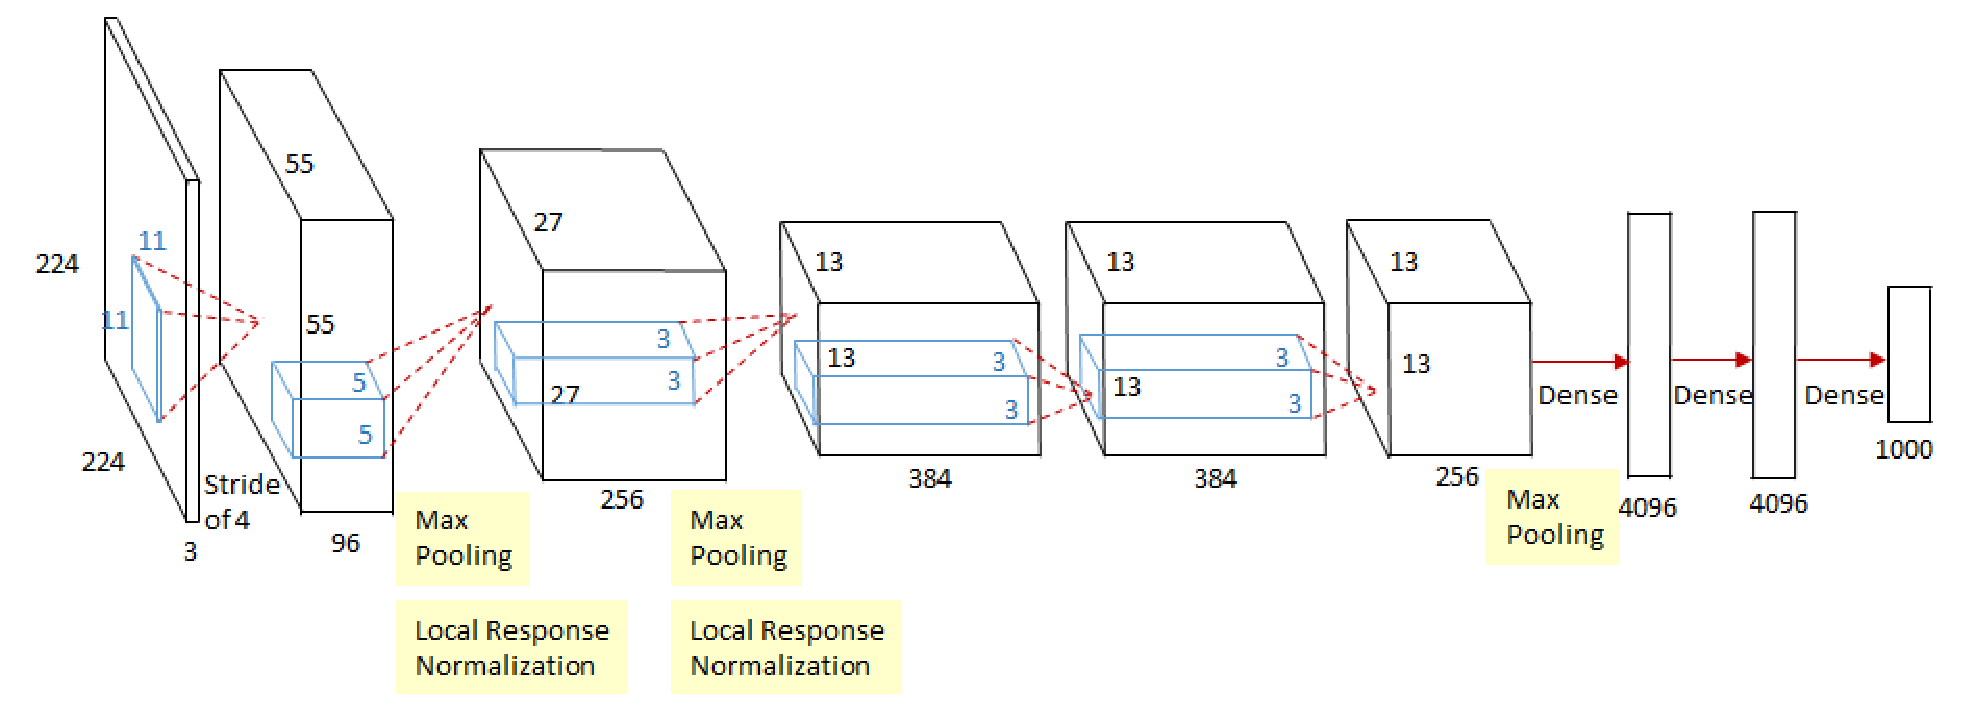
\includegraphics[width=\linewidth]{fig/caffenet.eps}
    \caption{Layer configuration of CaffeNet \cite{reviewalex}}
    \label{fig:caffenet}
\end{figure}

\subsection{Base FPGA implementation}

This section shows the implementation used on the first iteration of the CaffeNet neural network.
Each of the layers were implemented as OpenCL kernels that the compiler transforms into a binary
file that can be used to reprogram the FPGA directly from the Yocto Linux distribution ran
on the ARM Cortex-A9 processor.

\subsubsection{Host code}

The host code is developed using C++, following common \intelOCL examples. The code for this
project is in charge of inserting the training weights file into each of the layers of the
FPGA, as well as resizing the images to fit the 224{x}224{x}3 requirement. The code is capable
of processing only images with .jpeg or .jpg extensions and accepts directories in order to
process a batch of images.

After finishing evaluating each of the images, the code retrieves the values of the output 
matrix in the FPGA and prints to the screen the final classification, including up to the first 
5 possibilities in order to properly evaluate top-1 and top-5 accuracy.

\subsubsection{Convolution layer}

As specified on \cite{suda}, the convolution layer performs a series of 3-dimensional multiply and accumulate (MAC)
operations. These operations can be simplified by using flattening and rearranging of the input features. This way,
the MAC operations end up being simple multiplications that are accumulated and sent to the output buffer.

The general algorithm is as follows:
\begin{enumerate}
    \item Compute the address locations of the input and kernel matrixes
    of the specific work-item identifier.
    \item Load the kernel and input 2-D matrixes into local memory. The input is loaded
    as input[x][y] and the kernel/weights is loaded as kernel[y][x].
    \item Apply the MAC operation as follows: 
    
    output += kernel[y][k]*input[x][k]
    \item Wait until all work-items finish the work.
    \item Save the output to the output buffer using the SDK channels.
\end{enumerate}

These steps must be repeated for every neuron. This process can be optimized using OpenCL
pragma directives to allow for Single Instruction Multiple Data (SIMD) processing. The
parameters that define the convolution layer can be seen in Table \ref{table:convlayer}.
Static parameters are defined for every layer, while dynamic ones are defined per layer
using a JSON description of the network.

The stride and pad are used to determine the index of the input matrix.
Also, each kernel uses a local memory buffer to store the results of each operation.
The buffer size is modified by the SIMD factor, as doing multiple operations at
once requires multiple sections of memory.

\begin{table}[H]
    \begin{center}
        \caption{Parameters used on the convolution layer.}
        \begin{tabular}{lll}
        \hline
        Value                 & Type    & Usage                           \\ \hline
        CHANNEL\_N\_VECTORIZE & Static  & MAC SIMD factor                 \\
        CHANNEL\_N\_WIDTH     & Static  & Neuron SIMD factor              \\
        CONV\_CH\_SIZE\_BUF   & Static  & Local memory buffer             \\
        CONV\_CH\_SIZE\_BUF   & Static  & Local memory buffer             \\
        CONV\_CH\_STRIDE      & Dynamic & Stride to use per layer         \\
        CONV\_CH\_PAD         & Dynamic & Padding to add to input feature \\ \hline
        \end{tabular}
        \label{tab:convlayer}
    \end{center}
\end{table}

\subsubsection{Pooling}

The pooling layers are implemented using overlapping max pooling, following AlexNet's
configuration. This means that the kernel downsample the input by selecting the maximum
value of each input window matrix and the stride used results in overlapping results.

The algorithm is a simple iteration over each of the values of the window and selecting
the maximum. The parameters used in this type of layer are shown in Table \ref{table:poolinglayer}
The SIMD factor determines the size of the local memory to be used.

\begin{table}[H]
    \begin{center}
        \caption{Parameters used on the pooling layer.}
        \begin{tabular}{lll}
        \hline
        Value                 & Type    & Usage                   \\ \hline
        CHANNEL\_N\_WIDTH     & Static  & Neuron SIMD factor      \\
        CONV\_SIZE\_BUF       & Static  & Local memory buffer     \\
        POOL\_CH\_EXTEND\_MAX & Static  & Local memory buffer     \\
        POOL\_EXTEND          & Dynamic & Internal SIMD factor    \\
        POOL\_STRIDE          & Dynamic & Stride to use per layer \\ \hline
        \end{tabular}
        \label{tab:poolinglayer}
    \end{center}
\end{table}

\subsubsection{Normalization}

Local response normalization (LRN) is applied using the formula described in
section \ref{theorylrn}. The algorithm followed to compute normalization for
each kernel is the following:

\begin{enumerate}
    \item For each \textit{input\_feature i}:
    \item For each neuron \textit{j} in feature \textit{i}:
    \item Compute \textit{sum\_of\_squares[j] += input\_feature[i+n/2][j]}
    \item Compute \textit{output\_feature[i][j] = input\_feature[i][j]*pwlf(k+$\alpha$*sum\_of\_squares[j])}
    \item Update \textit{sum\_of\_squares[j] –= input\_feature[i–n/2][j]}
\end{enumerate}

Where \textit{pwlf} is an approximate function with precomputed values. This
function is hard-coded to avoid doing the calculations in the FPGA and returns the value
of the exponential part of the equation in section \ref{theorylrn}. Exponential functions
are hard to implement hardware-wise, a version with approximate values using a dictionary
implemented directly as a ROM section is faster and provides the same functionality.

Table \ref{tab:normalizationlayer} shows the parameters used to configure the execution
of the normalization layer. Just like the other layers, a SIMD factor is used and can be
modified to increase the resource usage of the FPGA being used.

\begin{table}[H]
    \begin{center}
        \caption{Parameters used on the normalization layer.}
        \begin{tabular}{lll}
        \hline
        Value                  & Type    & Usage               \\ \hline
        CHANNEL\_N\_VECTORIZE  & Static  & Neuron SIMD factor  \\
        NORM\_N\_SLICES\_MAX   & Static  & Local memory buffer \\
        NORM\_SIZE\_IN\_MAX\_0 & Static  & Local memory buffer \\
        NORM\_N\_SLICES        & Dynamic & Memory access index \\
        NORM\_N\_SLICES\_MIN   & Static  & Internal SIMD factor \\ \hline
        \end{tabular}
        \label{tab:normalizationlayer}
    \end{center}
\end{table}

Normalization also allows for parallel SIMD operations. Each neuron can do its work
separate from the others and the normalization operation can also be applied in parallel
for each input feature slice. The slices determine how much work can be done per neuron
on each part of the input matrix.

\subsubsection{Fully Connected Layer}

The fully connected layer does the same work as the convolution layer, with the difference
that it is connected to every output from the layer before it. The parameters used are the
same.

\subsubsection{Activation Function}

AlexNet uses Rectified Linear Unit (ReLU) as the activation function. 
It is defined as f(x) = max(0,x) and it is applied after every convolution layer.
It allows to filter out negative values and provides non-linearity between layers. It also
has low computational complexity, as it is easy to implement.

% talk about channels if there is not enough pages

\subsection{Approximate changes}

Any approximate changed done in order to reduce the accuracy but improve the performance
and resource usage is described in the following sections.

\subsubsection{Arbitrary precision}

The fixed-point precision is defined for each layer on the JSON description of the network.
Each number contains an integer and fractional part, but are stored in the same variable.
To determine the bit length and position of the variable, a simple notation is used: 
\textit{[l,p]}, where \textit{l} is the length and \textit{p} is the position of the decimal
point from right to left.

The main objective of using lower precision values for different layers is to reduce the
resources needed in order to execute the network in the FPGA.

As an example, the decimal value 3.25 can be represented using the notation \textit{[5,3]}.
This yields the following binary number:

$$
11_2.010_2
$$

Fixed-point precision can change from the input of one layer to its output. This is achieved
by aligning the precision before applying the specific operation. The limitation is that the
input precision of a layer must match the output precision of the layer before it.m

Aside from manually implementing fixed-point precision, \intelOCL allows for implementation
of compilable arbitrary precision integers. Listing \ref{code:arbitrary} shows a simple
multiplication of two 7-bit integers, the result being saved into a 14-bit integer. The
compiler automatically assigns the desired amount of bits for each variable.

\begin{lstlisting}[language=C++, caption=Arbitrary precision integers, yielding
a 14 bit result, label=code:arbitrary]
// Intel FPGA arbitrary precision integers
uint7_t a2, b2;
uint14_t c2;
c2 = a2 * (uint14_t)b2;
\end{lstlisting}

\subsubsection{Approximate operations}

A CNN spends most of its computational resources on operations within the layers. These operations
can be changed to an approximate version of themselves. Some of the approximations used are:

\begin{itemize}
    \item Approximate MAC: using Adams \cite{adams2019energy} implementation of an energy-efficient
    and approximate MAC unit, gains in resource usage are expected. The execution time changes
    are unknown as Adams did not measure this specific parameter.
    \item Faster pooling operation: pooling operation iterates over the input matrix
    looking for the maximum value on each window. A faster operation can ignore specific
    values or skip loop iterations.
\end{itemize}

\subsubsection{OpenCL compiler optimizations}

OpenCL offers optimizations that promise increases in performance at the cost of accuracy.
This optimizations are set on compile time and are specific to OpenCL, not Intel's implementation
for the FPGA. The main approximations used are:

\begin{itemize}
    \item -fp-relaxed: relaxes the order of arithmetic operations. This is only applied 
    to operations on which the order does not affect the end result.
    \item -fpc: Removes intermediary roundings and conversions when possible, 
    and changes the rounding mode to round towards zero for 
    multiplies and adds.
    \item -cl-mad-enable: changes MAC operations to a mad. This is an approximate version of
    MAC with reduced accuracy.
\end{itemize}

There is no control on where these optimizations are applied, as it is set for the whole
compilation process.

\subsubsection{Memoization}

Memoization is applied mainly on convolution layers with small stride values. This is because
the objective is to approximate the overlapping calculations for each neuron. This is achieved
by skipping every other loop call in the main convolution functionality and using the latest
result as the output for every skipped iteration.

\subsubsection{CNN definition changes}

Some approximations that can be applied to the CNN are changing the configuration of the network
in order to reduce the amount of computation done or approximate its results.

\begin{itemize}
    \item Reduction of filter size: AlexNet uses 11{x}11 filters on the first layer. This size
    can be modified to a lower number in order to reduce the number of operations and the
    resource usage of the network. Another
    possibility is to change to specific constant values some of the iterations in the calculations.
    \item Increasing stride value: similarly to memoization, a bigger stride results in big gains
    on computation speed. This change should not affect the resource usage.
    \item Removal of layers: AlexNet achieves its low error-rate by increasing the number of layers
    in its definition. But a higher error-rate with gains in performance and resource usage is
    possible by reducing the depth of the network. This change can only be applied to the later
    layers, as a propagation from the initial layers would require retraining the network, which
    takes longer than the allocated time for the project.
\end{itemize}

\subsection{Validation and measurements}

The methods used to measure and validate the accuracy gains and losses, as well as the
improvement or degradation on performance and resource usage are described in the following
sections.

\subsubsection{Accuracy}

The original validation set used by AlexNet consists of 120000 images from 1000 classes.
Due to limitation in time, the set used in the project consists of only 4000 images.
Accuracy is measured against top-1 and top-5 classification. Each image has a specific class
assigned to it and the validation process returns a matrix with possibilities
for each class.

A Python 3.5 script is used in order to evaluate the validation results of each compiled
CNN against the expected results. The process is a counting of \textit{hits} (good results) for
the first class (top-1) and counting of \textit{hits} for the first 5 classes (top-5).

The actual error-rate is calculated as follows:

$$
Top1_{error} = \frac{\#images - \#top1_{hits}}{\#images}
$$
$$
Top5_{error} = \frac{\#images - \#top5_{hits}}{\#images}
$$

\subsubsection{Performance}

After the input image is resized and transformed into the input matrix, the start time
is measured and when the process is finished, the end time is measured again. The difference
between both times is used as the execution time of the network.

\subsubsection{Resource usage}

\intelOCL provides HTML reports of the estimated resource usage during and after compilation time.
The report contains information on the usage of the following resources:
\begin{itemize}
    \item Adaptive look-up tables (ALUTs): represent the percentage of
    available logic resources used in compiled designed. Each adaptive logic module (ALM)
    can be used to implement two ALUTs.
    \item Registers (FFs): represent the rest of the logic implementation within the
    FPGA.
    \item Digital signal processing units (DSPs): specialized DSP units used by the FPGA
    on complex operations.
    \item Random access memory (RAMs): local memory available within the FPGA. No external RAM
    is being used for this project, so this percentage represents the actual memory usage
    of the whole network.
\end{itemize}

All of these resources should go down when implementing approximate versions of the CNN.

\section{Results and analysis}

\subsection{Error tolerance}

\subsection{Resource usage}

\subsection{Performance}
  \chapter{Conclusions and recommendations}

In the next section, the main discoveries of the project are
presented. Also, some recommendations are given on what
future projects can focus on and how the current work
can be expanded.

\section{Conclusions}

OpenCL can be used to describe approximate operations on neural networks through
the use of compiler flags and approximate algorithm
implementation. On CNN implementations, OpenCL allows
for high-level implementation of hardware definition with
performance gains and resource usage reductions.

Approximate computing techniques can be used
on CNNs to show their error-tolerance property. 
Iteration skipping and memoization 
on pooling layers had
the best results in terms of performance with a minimal accuracy loss.

One of the biggest advantages of using FPGA is being able to properly control
the precision of variables being used. Because of this, changing the precision
on arithmetic operations and input values represents significant reductions on resource
usage on FPGA implementations of CNNs.

The best accuracy-performance ratio found was an increase of 5.66\% on the top-1 error
with a performance gain of 4.39\%. This performance can be boosted
by increasing parallelism and maximizing the resource usage
of the FPGA. A combination of techniques could be used to achieve even 
lower execution times with different levels of accuracy.

\section{Recommendations}

The utilization of approximate computing techniques on FPGA-implemented
CNNs can be expanded through the combination of the different types
of techniques shown in this work. The current project's scope can
be expanded to show the maximum performance and resource usage gain
from approximate techniques.

OpenCL represents a good entry into the hardware definition area.
The project, however, could be expanded upon through the use of
low-level hardware definition languages such as Verilog to produce
finely-tuned approximate solutions.

The current project targeted a relatively low power FPGA. The use
of a more powerful platform could lead to better performance
in comparison to a CPU/GPU CNN implementation.

  %----------------------------------------------------------------------------
  % literature in bibtex way:
  % \bibliographystyle{sty/plainurl} % for english documents
  % \bibliography{literatura}
  % literature in biblatex/biber way
  \printbibliography[heading=bibintoc,title={Bibliography}]
  %----------------------------------------------------------------------------

  %----------------------------------------------------------------------------
  % \annex
  % \renewcommand{\appendixname}{Annex}
  \appendix
  %----------------------------------------------------------------------------

  \chapter{Implicaciones sociales y éticas del proyecto}

El presente proyecto busca aportar al área de investigación en
redes neuronales convolucionales. Este tipo de redes neuronales
es utilizado principalmente para el reconocimiento y clasificación
de imágenes. Esto implica que se puede determinar el contenido
de una imagen de la misma forma que el cerebro humano procesa
e identifica a la misma imagen.

Con el incremento en la generación de datos por medio
de múltiples dispositivos y la creciente tendencia de el "internet de las cosas",
existe una creciente responsabilidad de parte de la sociedad de utilizar
las redes neuronales convolucionales de forma beneficiosa para esta.
Sociedades actuales hacen uso de este tipo de aplicaciones como
forma de control de masas o para aumentar ganancias monetarias de
poderosas empresas.

Sin embargo, también existen usos positivos para el reconocimiento
de imágenes. En aplicaciones médicas, aeroespaciales, tecnológicas,
científicas
y más, es posible ver los beneficios que las redes neuronales tienen
para la sociedad en general. Se espera que este proyecto represente
un avance que pueda ayudar a mejorar la vida de las personas.

  %----------------------------------------------------------------------------
  \backmatter
  %----------------------------------------------------------------------------

  \printindex                % insert index into document. Don't forget to call
                             % "makeindex filename" first.
\end{document}
